\documentclass[12pt]{article}

\usepackage{upgreek}

\usepackage{amsmath}

\usepackage{graphicx}
\graphicspath{ {imgs/} }

\usepackage{enumitem}

\usepackage{listings}

\usepackage{mathtools}
\DeclarePairedDelimiter\ceil{\lceil}{\rceil}
\DeclarePairedDelimiter\floor{\lfloor}{\rfloor}

\usepackage{color}
 
\definecolor{codegreen}{rgb}{0,0.6,0}
\definecolor{codegray}{rgb}{0.5,0.5,0.5}
\definecolor{codepurple}{rgb}{0.58,0,0.82}
\definecolor{backcolour}{rgb}{0.95,0.95,0.92}
 
\lstdefinestyle{mystyle}{
    backgroundcolor=\color{backcolour},   
    commentstyle=\color{codegreen},
    keywordstyle=\color{magenta},
    numberstyle=\tiny\color{codegray},
    stringstyle=\color{codepurple},
    basicstyle=\footnotesize,
    breakatwhitespace=false,         
    breaklines=true,                 
    captionpos=b,                    
    keepspaces=true,                 
    numbers=left,                    
    numbersep=5pt,                  
    showspaces=false,                
    showstringspaces=false,
    showtabs=false,                  
    tabsize=2
}
 
\lstset{style=mystyle}

\usepackage{dsfont}

\usepackage{hyperref}

\usepackage[utf8]{inputenc}

\usepackage{mathtools}

\usepackage{textcomp}

\usepackage[english]{babel}

\usepackage{tikz}

\usepackage{tcolorbox}

\usepackage{amsthm,amssymb}

\setlength{\parindent}{0cm}

\renewcommand\qedsymbol{$\blacksquare$}

\usepackage{fancyhdr}
 
\pagestyle{fancy}
\fancyhf{}
\fancyhead[LE,RO]{Algorithm Design and Analysis -- Fall 2017}
\fancyhead[RE,LO]{Joshua Concon}
\fancyfoot[CE,CO]{\leftmark}
\fancyfoot[LE,RO]{\thepage}


\begin{document}

\title{CSCC73: Algorithm Design and Analysis\\ Lecture Notes}
\date{University of Toronto Scarborough -- Fall 2017}
\author{Joshua Concon}
\maketitle
Pre-reqs are CSCB63 and STAB52.
Instructor is Dr. Vassos Hadzilacos. He projects well so you can basically sit anywhere. If you find any problems in these notes, feel free to contact me at conconjoshua@gmail.com.

\tableofcontents

\pagebreak

\section{Wednesday, September 6, 2017}

\subsection{Greedy Algorithms}

All Greedy Algorithms are \underline{Optimization problems:} given input, compute output that
\begin{enumerate}
	\item{satisfies constraints}
	\item{optimizes (min or max) certain criteria}
\end{enumerate}

Solutions that satisfies constraints are called \textbf{feasible}.

\subsubsection{Interval Scheduling (KT 4.1)}

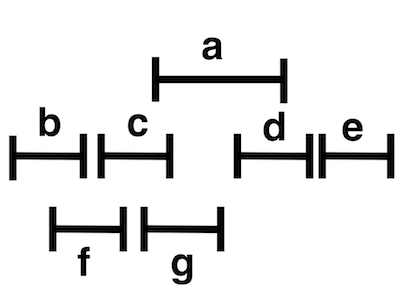
\includegraphics{interval1}\\
\\
\underline{Input:} Set of jobs $1,2,...,n$ where job $i$ has start time $s(i)$ and finish time $f(i) > s(i)$

\begin{tcolorbox}
	jobs $i,j$ conflict if each starts before the other finishes. i.e. if $s(i) < f(j)$ and $s(j) < f(i)$
\end{tcolorbox}

\underline{Feasible set of jobs:} A set where no two jobs conflict.\\
\\
\underline{Output:} A max cardinality feasible set (a max non-conflicting set of jobs) ('a set' rather than 'the set' as there may be more than 1 optimal sets.)\\
\\
\underline{e.g.} $\{ b,c,d,e \}, \{ b,g,d,e \}$ (from figure 1)\\
\\
\underline{Greedy "Schema":}\\
\begin{lstlisting}[language=Python]
sort jobs in some order
A := null
for each job i in sorted order do
	if i conflicts with no job in A then
		A := union of A and {i}
return A
\end{lstlisting}

We will make edits to this schema as we learn more about what sort order provides us with the most optimal set.

\subsubsection{Possible sort orders}

\begin{enumerate}
	\item{
	\textbf{sort by increasing start time}\\
	counterexample:\\
	\\
	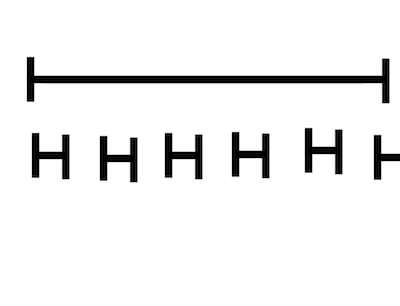
\includegraphics{interval2}\\
	\\
	As shown in the picture, the most optimal answer are the short intervals that come after the long interval has started, but the long interval is chosen first conflicting with the rest of the intervals.
	}
	\item{
	\textbf{sort by increasing duration length}\\
	counterexample:\\
	\\
	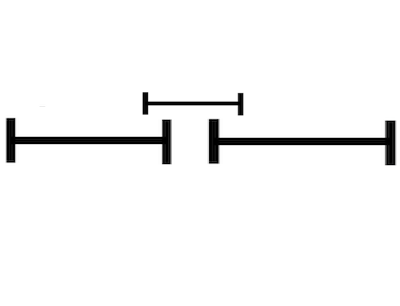
\includegraphics{interval3}\\
	\\
	The optimal answer in this picture is the two long intervals, but since there shorter interval is chosen and it conflicts with both of the long intervals, this sort does not work.
	}
	\item{
	\textbf{sort by increasing number of conflicts}\\
	counterexample:\\
	\\
	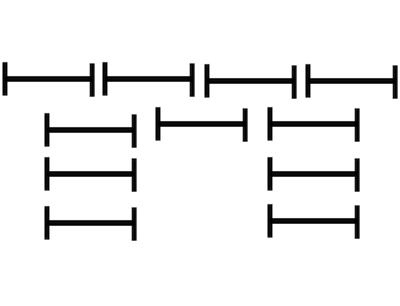
\includegraphics{interval4}\\
	\\
	In this case, the most optimal answer is all 4 of the top intervals. However, since it starts with the interval with the least amount of conflicts, it chooses an interval that conflicts with 2 of the 4 top intervals, which is the middle interval.
	}
	\item{
	\textbf{sort by increasing finish time}\\
	this increments $A$ using the smallest amount of time as possible, and this is also the correct sort for this algorithm.
	\\
	}
\end{enumerate}

\underline{Greedy "Schema" Revised:}\\
\begin{lstlisting}
sort jobs in increasing finish time
A := null
F := -infinity
for each job i in sorted order do
	if s(i) >= F then
		F := f(i)
		A := union of A and {i}
return A
\end{lstlisting}

\underline{Running Time:} $O(nlogn) + O(n) + O(1) = O(nlogn)$

\subsubsection{Proof of Correctness (optimality)}

Let $j_1, j_2, ... , j_k$ be jobs added to A in order considered

\paragraph{Claim 1:} A is feasible, proof trivial (just use sort by increasing finish time in the scheme, nothing in A should conflict by the algorithm).\\
\\
Let $j_1^*, j_2^*, ... , j_m^*$ be jobs in some optimal $A^*$ (in left to right order)
\paragraph{Claim 2:} $f(j_t) \leq f(j_t^*), \forall t, 1 \leq t \leq k$ (greedy algorithm stays ahead)

\begin{proof}
(proof of Claim 2)\\
Use induction.\\
\\
\underline{Basis:} $t=1$, algorithm adds interval with earliest finish time to $A$, so this holds.\\
\\
\underline{Induction Step:} For contradiction, assume $f(j_{t+1}) > f(j_{t+1}^*)$. This is immpossible because $f(j_t) \leq f(j^*_t)$ and the Induction Hypothesis Algorithm has not considered $j^*_{t+1}$ yet and will consider $j^*_{t+1}$ before $j_{t+1}$ and will add $j^*_{t+1}$ to $A$ instead of $j_{t+1}$.\\
\\
\underline{Induction Hypothesis:} $f(j_t) \leq f(j^*_{t})$\\
\\
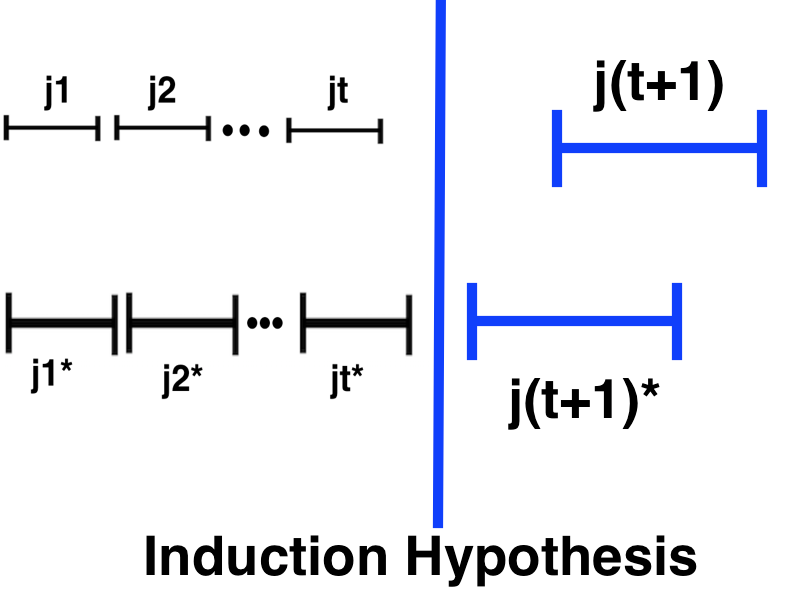
\includegraphics{interval5}\\
\\
Assume for contradiction: $f(j_{t+1}) > f(j_{t+1}^*)$.\\
\\
We have... 
\begin{align*}
	f(j_t) &\leq f(j_t^*)\:\:\:\text{by Induction Hypothesis}\\
	&\leq s(j_{t+1}^*)\:\:\:\text{Because $A^*$ is feasible and jobs are labelled left to right}\\
	&< f(j_{t+1}^*)\:\:\:\text{Finish time is strictly greater than start time}
\end{align*}

Immediately after the algorithm adds job $j_t$ to $A$, job $j^*_{t+1}$:
\begin{itemize}
	\item{has not been considered $(f(j_t) < f(j^*_{t+1})$}
	\item{$j^*_{t+1}$ does not conflict with jobs in $A$ as $f(j_t) \leq f(j^*_t) \leq s(j_{t+1}^*)$}
	\item{$j^*_{t+1}$ has priority over $j_{t+1}$ (by assumption, $f(j_{t+1}) > f(j^*_{t+1})$)}
\end{itemize}

Therefore $j_{t+1}$ is not the next job added to $A$ by the algorithm, therefore there is a contradiction. So Claim 2 must be true.

\end{proof}

\paragraph{Claim 3:} $k=m$

\begin{proof}(Proof of Claim 3)\\

Clearly $k\leq m$, since m is optimal.\\
Assume for contradiction that $k < m$\\
\\
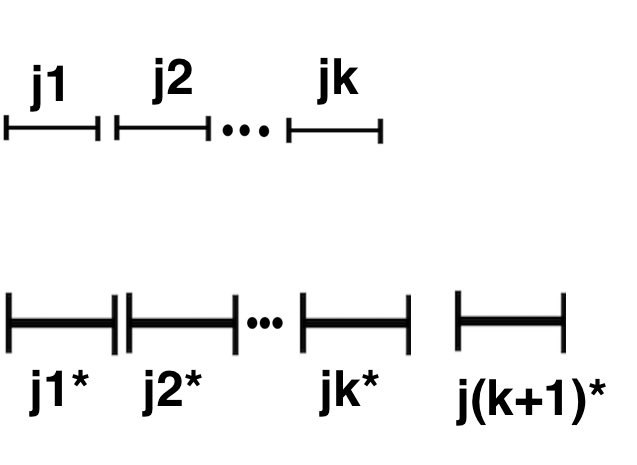
\includegraphics{interval6}\\
\\
But then $j^*_{k+1}$ should also be in $A$, but it's not in $A$. Therefore it doesn't exist.\\
\\
Therefore $k=m$
\end{proof}

\underline{Alternative Approach ("promising set"):}\\
For each iteration $i$ in a Greedy Algorithm, there exists an optimal set $A^*$ such that $A_i \subseteq A^*$\\

\underline{Generalization of Interval Scheduling:}\\
Interval Scheduling can be generalized to cover different problems, such as Weighted Intervals, finding the minimum amount of concurrent machine to perform all intervals.

\newpage

\section{Monday, September 11, 2017}

\subsection{Min-Max Lateness (KT 4.1)}

\underline{Input:}
\begin{itemize}
	\item{release time $r$ (earliest time to start all jobs)}
	\item{$n$ jobs $1,2,...,n$}
	\item{for each job $i$}
	\begin{itemize}
		\item{length $t(i) \geq 0$}
		\item{deadline $d(i)$}
	\end{itemize}
	\item{can only do jobs one at a time}
\end{itemize}

We want to minimize the maximum lateness of any job.\\
\\
\underline{Schedule:} $S$ specifies start time of each job $i$. $(s(i) \geq r)$\\
\\
end time of $i = s(i) + t(i)$, such that $[ s(i), s(i)+t(i) ]$ and $[ s(j), s(j)+t(j) ]$ do not overlap for all jobs $i,j$ where $i \neq j$\\
\\
\underline{Output:} Find an $S$ that minimizes the max lateness of any job.\\

\textbf{Example:}

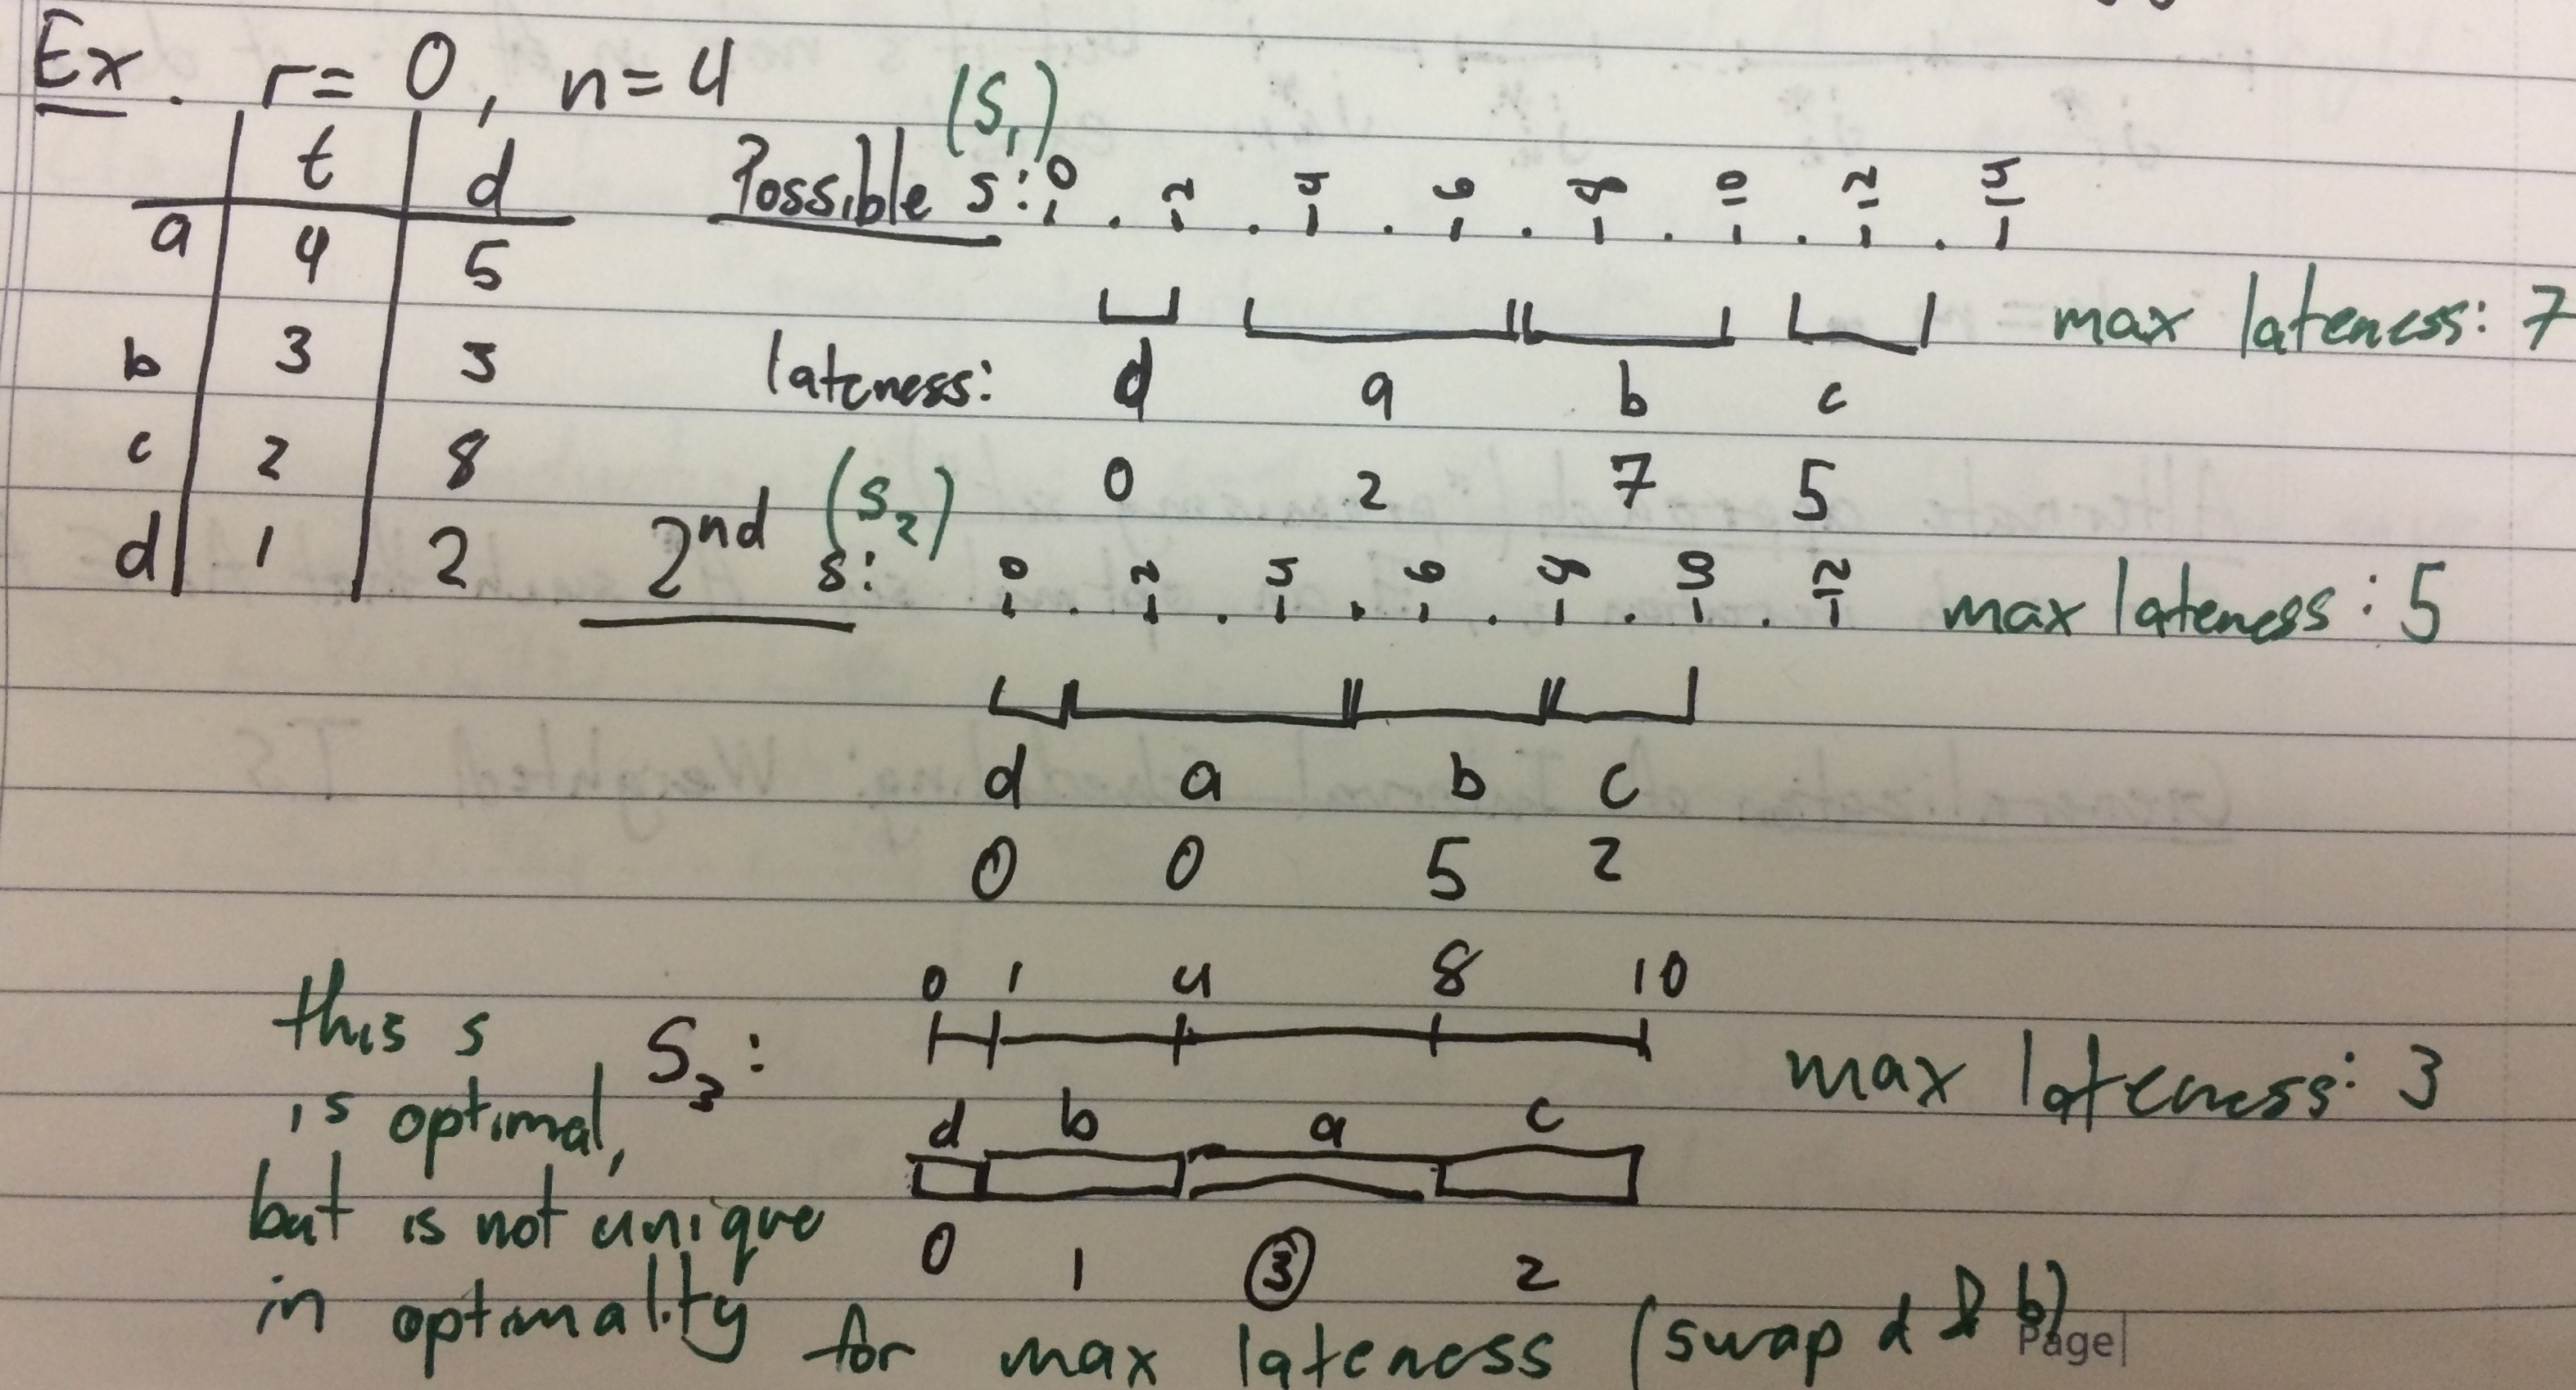
\includegraphics[scale=0.15]{minmax1}

This $S$ is optimal, but is not unique in optimality for the smallest max lateness (you can get another optimal solution by swapping $d$ and $b$)\\

\underline{Algorithm (Earliest Deadline First):}

\begin{lstlisting}[language=Python]
ALGO:
	Sort jobs by increasing deadline
	Let d[1,..,n] be deadlines (in sorted order)
	Let t[1,...,n] be durations of corresponding jobs
	F := r # max finish time of all jobs schedules so far
	for i:= 1 to n do
		gs(i) := F
		F := gs(i) +t (i)
	return gs
\end{lstlisting}

\underline{Running Time:} $\Theta (nlogn)$\\
\\
\begin{tcolorbox}[title=Inversion]
	An \textbf{inversion} in schedule $S$ is a pair of jobs $i,j$ such that $s(i) < s(j)$ but $d(i) > d(j)$\\
	\\
	\underline{i.e.}\\
	 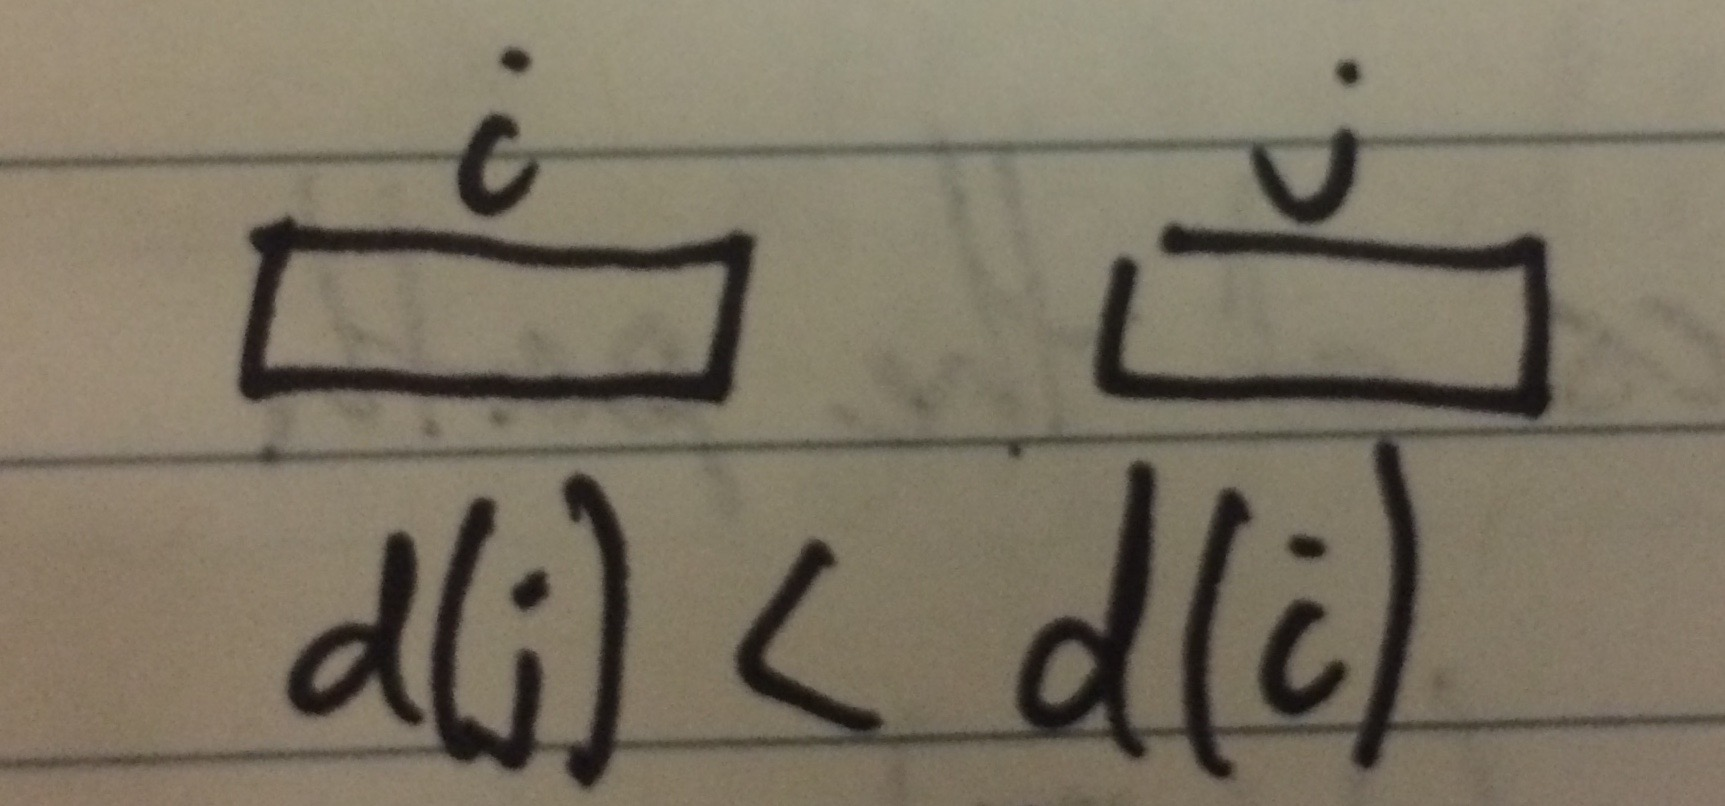
\includegraphics[scale=0.1]{minmax2}
\end{tcolorbox}

This algorithm has no gaps and no inversions, which both properties ensures optimality.\\
\\

\begin{tcolorbox}[title=Theorem]
	Any schedule with no gaps and no inversions is optimal
\end{tcolorbox}

\underline{Observation 1:} There is an optimal schedule with no gaps\\
\\
\underline{Observation 2:} All schedules with no gaps or inversions have the same max lateness\\
\\
Given $S$ with no gaps and at least 1 inversion, there exists a pair of jobs $i,j$ that have an inversion and are consecutive in s.\\
\\
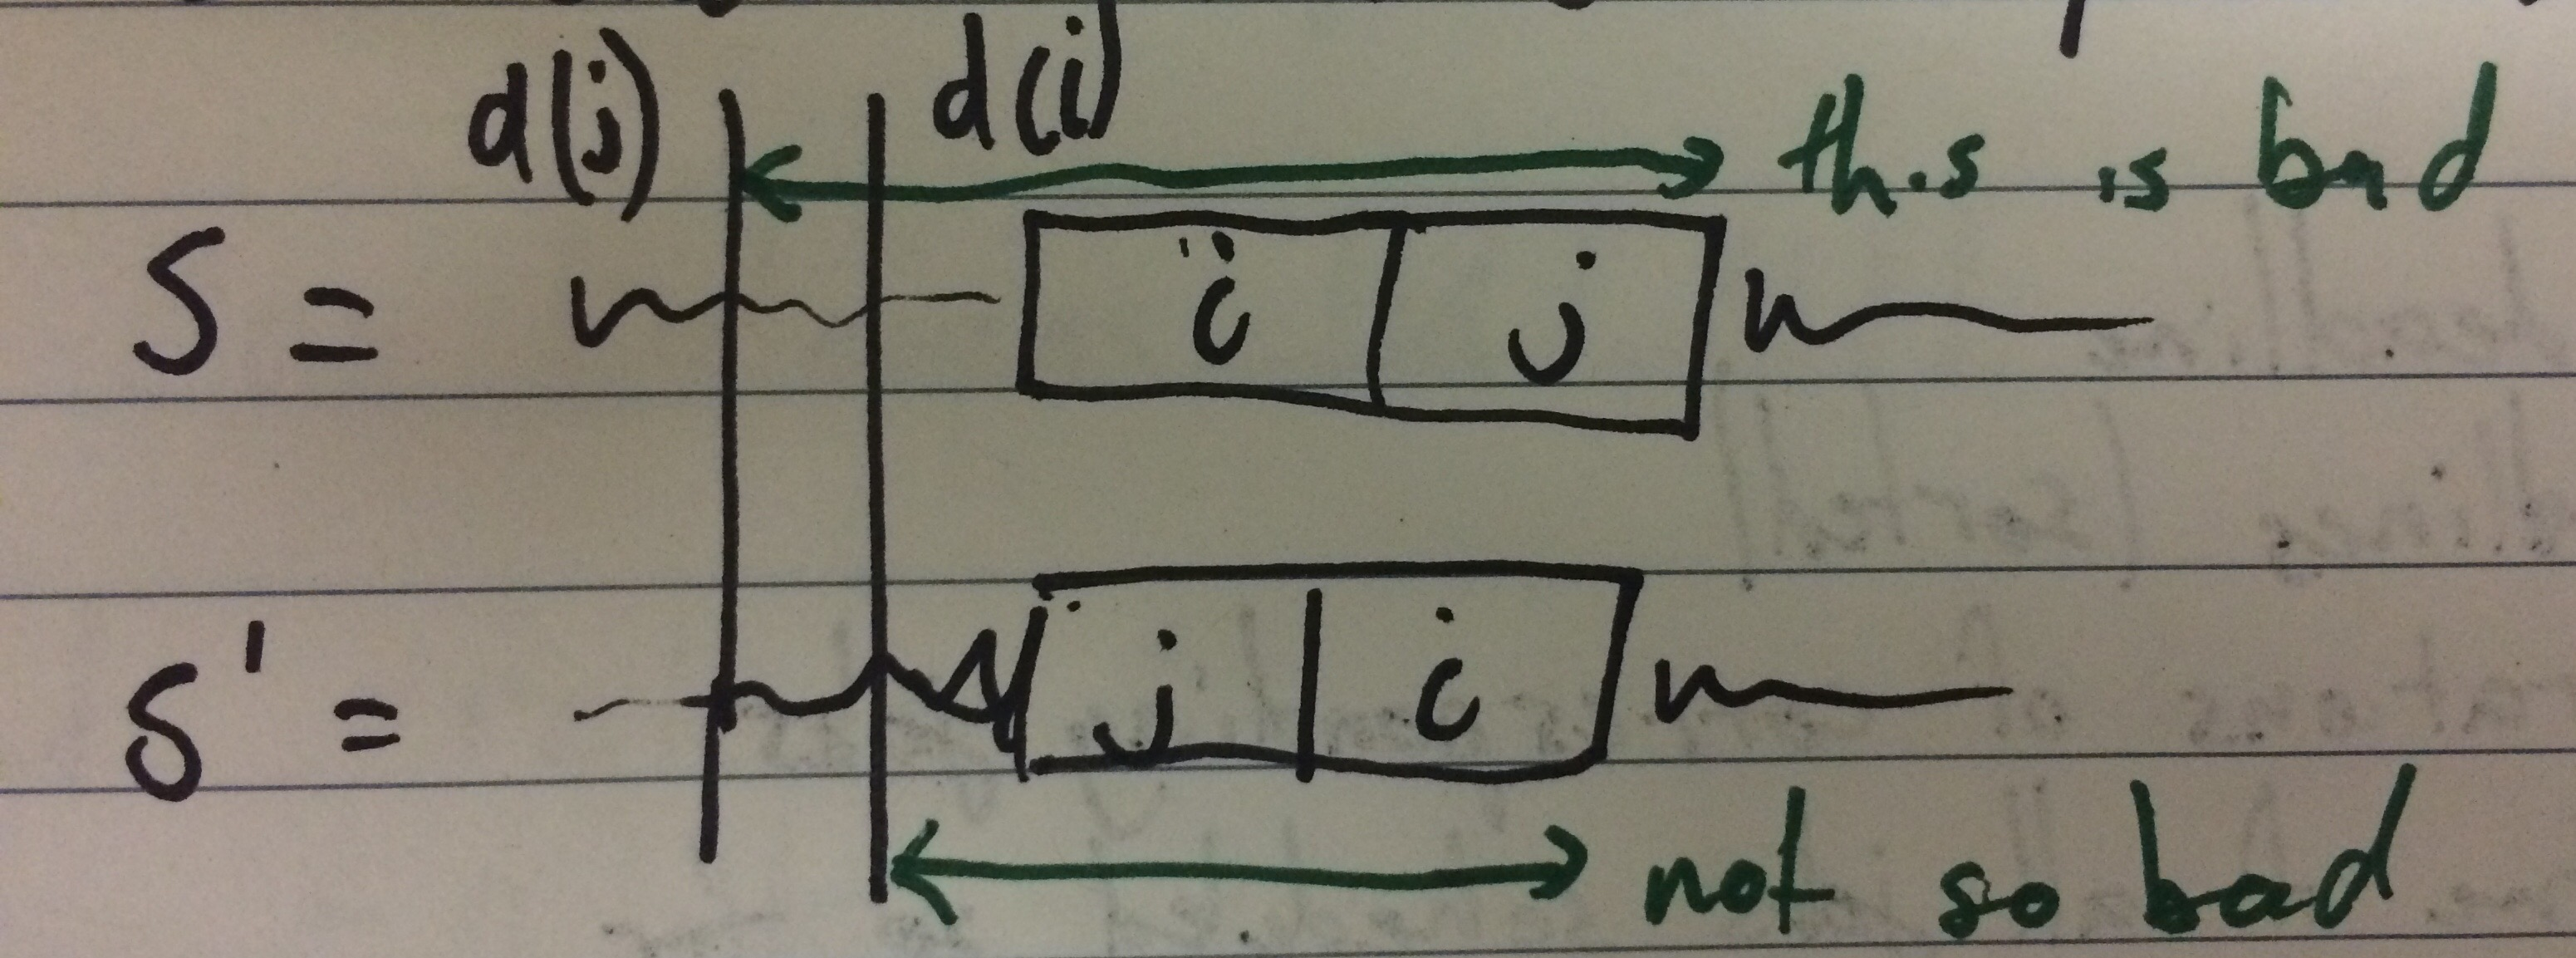
\includegraphics[scale=0.11]{minmax4}
\\
\\
Let $S'$ be a schedule like $S$ except $i,j$ are swapped.\\
\\
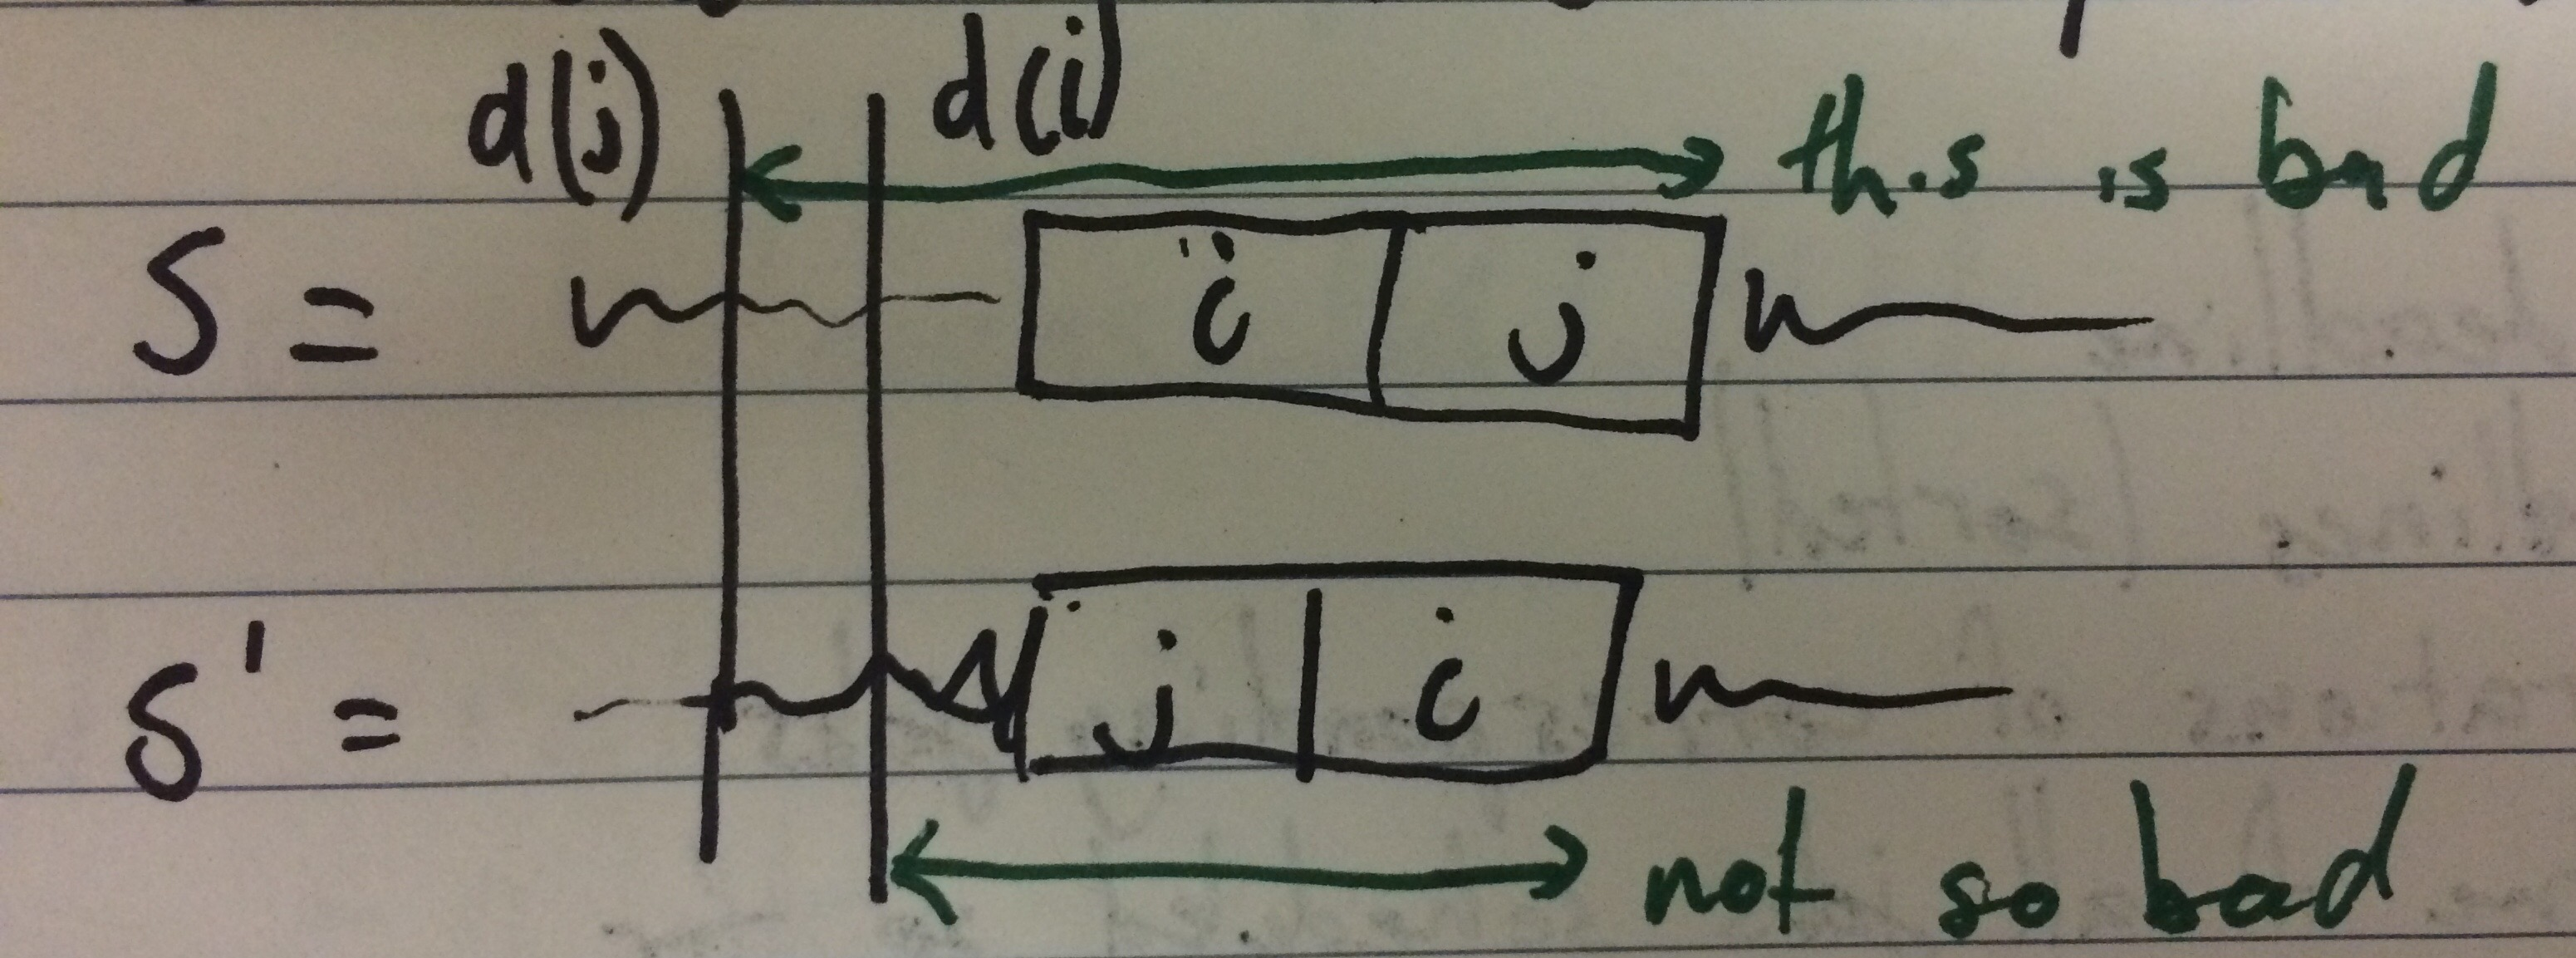
\includegraphics[scale=0.11]{minmax4}
\\
\\
\begin{itemize}
	\item{All jobs that are not $i,j$ have the same lateness in $S$ as in $S'$}
	\item{Lateness of $j$ in $S'$ does not increase}
	\item{Lateness of $i$ in $S'$ may increase though, but less than lateness of $j$ in $S$}
\end{itemize}
This implies that the max lateness in $S'$ $\leq$ max lateness in $S$.

\newpage

\section{Wednesday, September 13, 2017}

\subsection{Dijkstra's Shortest Path Algorithm (KT 4.4, DPV 4.4)}

$wt(P) = $ sum of the weights of edges of the path $P$\\
\\
\underline{Input:} 
\begin{itemize}
	\item{Weighted (di)graph $(G=(V,E))$}
	\item{source node $s\in V$}
	\item{weight of edges $wt(u,v) \geq 0, \forall (u,v) \in E$}
\end{itemize}

\underline{Output:} $\forall v \in V$
\begin{itemize}
	\item{$\delta (v) = $ minimum weight of $s \rightarrow v$ path}
	\item{$p(v) = $ predecessor of $v$ on a shortest $s \rightarrow v$ path}
\end{itemize}

We must maintain a set of nodes $R$, and $\forall u\in V, d(u)$

\underline{Intervals:}
\begin{enumerate}
	\item{$\forall u\in V, d(u) = $ minimum weight of any $s \rightarrow u$ path in which all nodes that are not $u$ are in $R$ ("$R$ - path")\\
	\\
	\underline{Visualization:}\\
	\\
	(insert pic here)
	\\
	\\
	or $d(u) = \infty$, if no such path exists}
	\item{$\forall u \in R, \forall u' \not\in R, d(u) \leq d(u')$}
\end{enumerate}

\underline{Note:}
\begin{itemize}
	\item{$\forall u, d(u) \geq \delta (u)$}
	\item{$\forall u \in R, d(u) = \delta (u)$}
\end{itemize}

\subsection{Algorithm}

\begin{lstlisting}[language=Python]
ALGO:
	R := {s}
	d(s) := 0
	p(s) := NULL
	for each node u != s do
		if (s,u) in E then
			d(u) := wt(s,u)
			p(u) := s
		else
			d(u) := infinity
			P(u) := NULL
	while R != V do
		let v be node not in R such that d(v) is min
		R := UNION(R,v)
		for each node u such that (v,u) in E do
			if d(u) > d(v) + wt(v,u)
				d(u) := d(v) + wt(v,u)
				p(u) := v
\end{lstlisting}

\underline{Visualization:}\\
\\
(insert pic here)

\subsection{Running Time}

($n = |V|, m = |E|$)

\begin{enumerate}
	\item{ \underline{Native Implementation:} $O(n) + O(n)O(n) = O(n^2)$\\
	\\
	The first $O(n)$ from the left is the running time for the initialization of all nodes before the while loop begins, the second $O(n)$ refers to how many times the while loop runs, and the last $O(n)$ refers to how long each loop takes. This results in a running time of $O(n^2)$}
	\item{ \underline{"Sophisticated" Implementation:}\\ $O(n) + O(n) + O(nlogn) + O(mlogn) = O((n+m)logn)$ or $O(mlogn)$ if it is assumed that there are no unreachable nodes from $s$}\\
	\\
	The first $O(n)$ refers to the initialization of all nodes before the while loop begins, the second $O(n)$ refers to the execution of BUILDHEAP on the nodes, the $O(nlogn)$ refers to the $O(n)$ EXTRACTMIN operations from this heap, and $O(mlogn)$ refers to all the change key operations for this heap.
\end{enumerate}

$O(n^2)$ vs. $O(mlogn)$, worst case $m = n^2$ (all nodes are connected to a linear amount of nodes).\\
\\
if $G$ is "dense" (i.e. $m = \Theta (n^2)$) then naive is faster\\
if $G$ is "sparse" then it's the opposite

\underline{Why non-negative weights for the edges?}\\
\\
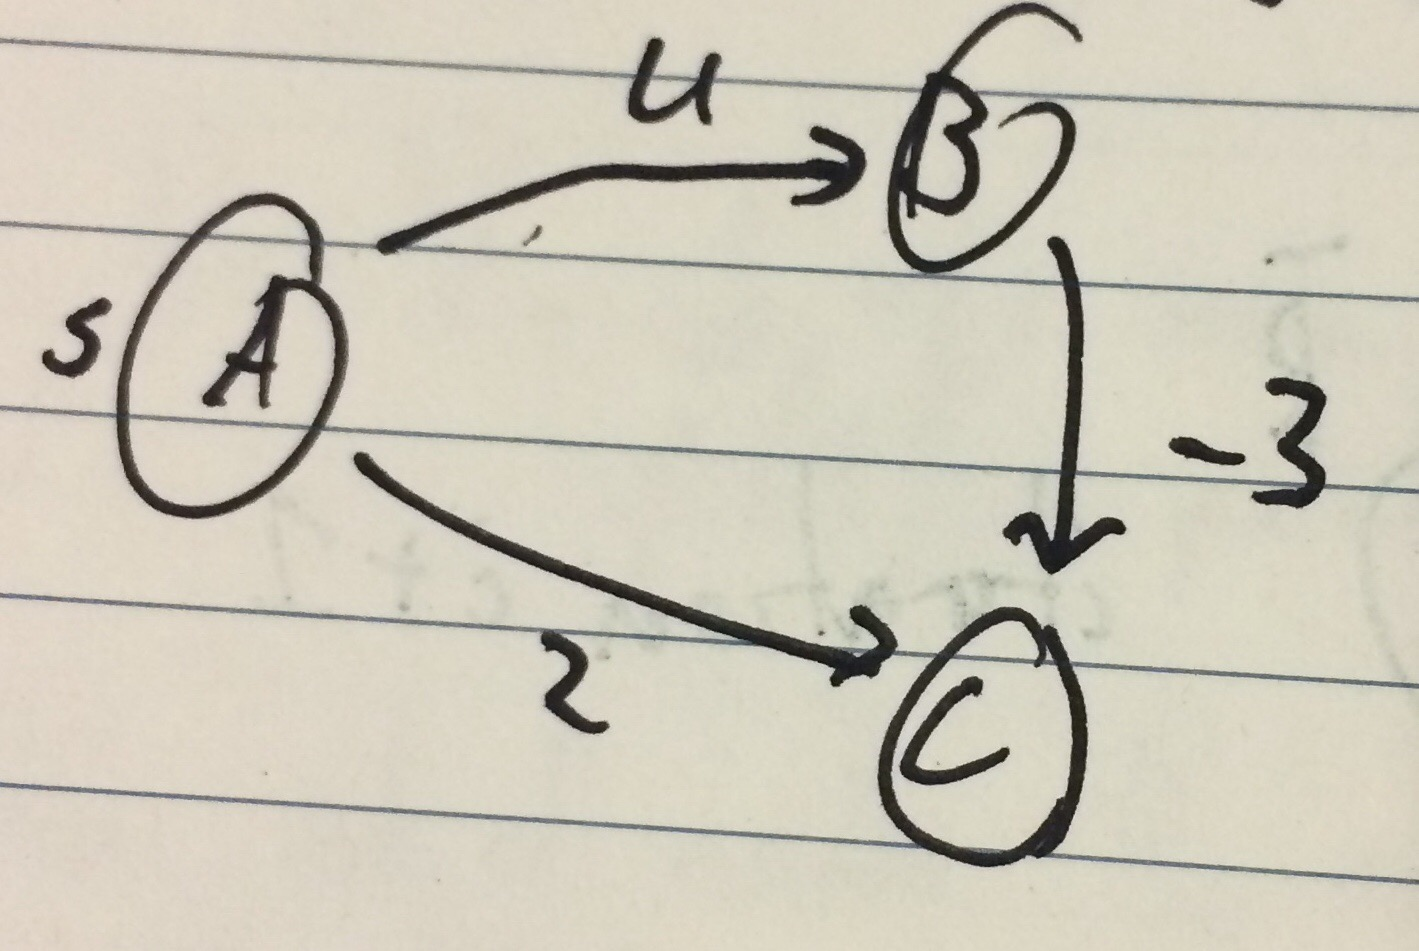
\includegraphics[scale=0.25]{lec3-1}
\\
\\
With $s = A$, the fastest route to $C$ from $A$ is $A \rightarrow B \rightarrow C$ which is wrong.

\subsection{Correctness}

$R_i, d_i = $ values of $R,d$ at the end of $i$th iteration.

\paragraph{Claim 1:} If invariants $(1)$ and $(2)$ hold. $\forall u \in R_{i+1}, d_i (u) = \delta (u)$\\
(\underline{Note:} $R_{i+1} = R_i \cup \{ v \}$)

\begin{proof}
	(Proof of Claim 1:)\\
	Let $u \in R_i \cup \{ v \}$ and $P$ be a minimum weight $s \rightarrow u$ path.\\
	\\
	If $P$ is on $R_i$-path, then done by invariant (1)
	If $P$ is not on $R_i$-path...\\
	\\
	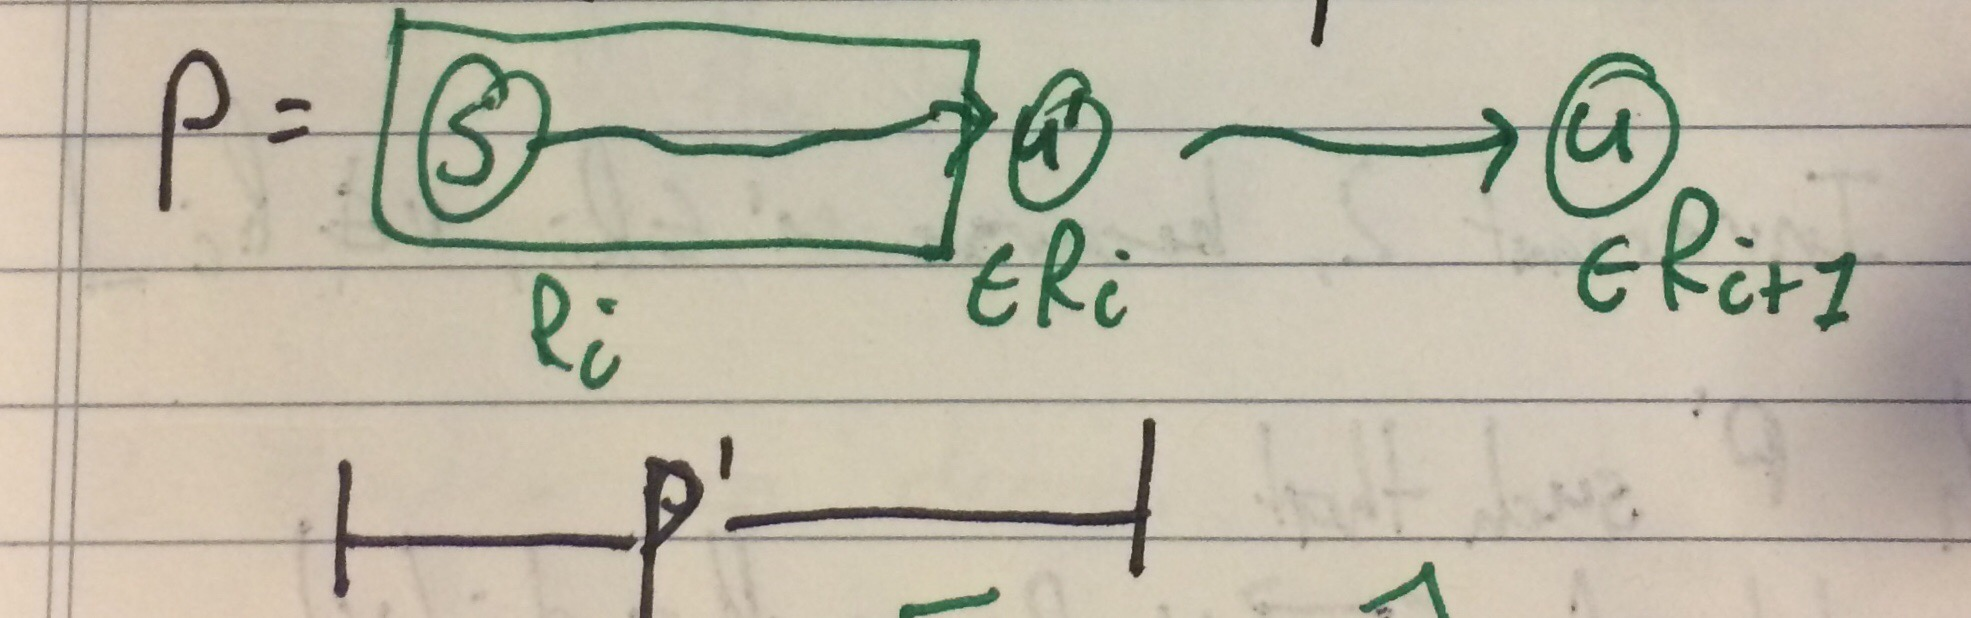
\includegraphics[scale=0.2]{lec3}
	\\
	\\
	Note how $u' \in R_i$, and $u \in R_{i+1}$
	\begin{align*}
		\delta (u) &= weight(P)\\
		&\geq weight(P') \:\:\:\text{since $wt \geq 0$}\\
		&\geq d_i (u') \:\:\:\text{by invariant 1, since $P'$ is an $s \rightarrow u'$ is an $R_i$ - path}\\
		&\geq d_i (u) \:\:\:\text{if $u\in R_i$ by invariant 2, $u=v$ by choice of $v$}\\
		&\geq \delta (u) \:\:\:\text{[since $\forall u, d(u) \geq \delta (u)$]}
	\end{align*}
	
	and this implies that $d_i (u) = \delta (u)$

\end{proof}

Why if invariants (1) and (2) hold after the $i$th iteration, invariant (1) holds after $(i+1)$st iteration for nodes $u \not\in R_{i+1}$\\
\\
Let $P$ be minimum-weight $s\rightarrow u$ $R_{i+1}$-path with the fewest occurrences of the new node $v$.\\
\\
\underline{Case 1: $v$ does not occur in $P$ at all}. This implies that $P$ is an $R_i$-path.

\begin{align*}
	&= minimum-weight\:\:\: s\rightarrow u\:\:\: R_{i+1}-path\\
	&= minimum-weight\:\:\: s\rightarrow u\:\:\: R_{i}-path\\
	&= d_i (u) \:\:\:\text{By the Induction Hypothesis}\\
	&= d_{i+1} (u)
\end{align*}

\underline{Case 2: $v$ occurs in $P$}\\
\\
Consider $R_i$, and there is an edge that connects a node from $R_i$ to a node $v$ outside of $R_i$, and there is yet another edge that connects that node $v$ to another node $u$, which is also outside of $R_i$. If $P$ is like this, then the algorithm computes a minimum-weight $s\rightarrow u$ $R_{i+1}$-path, so done.\\
\\
What happens if you get multiple instances of $v$ with are all outside $R_i$, so $R_i$ is divided into multiple sections because of the multiple instances of $v$ before having an edge connecting to a node in the most recent $R_i$ section to $u$?\\
\\
The answer is that this it can't happen, and here's why.
Consider the node in the most recent $R_i$ section that has an edge connecting to $u$, lets call this node $u'$.\\
\\
\underline{This node cannot be $v$}, as if it was, since the connections previous are non-negative, since there are multiple instances of $v$ and we are trying to find the minimum weight $s\rightarrow v$ path, then this case will not happen and would look more like case 2.
\\
\\
For contradiction, we are going to assume that this weird case where there are multiple instances of $v$ can happen, and that $u' \neq v$
$$d_i (u') \leq d_i (v)$$

We know this because $u' \in R_i$ and $v \not\in R_i$, do the $d_i$ value for $u'$ is smaller than the $d_i$ value for $v$ (so by invariant 2).\\

This implies that $\exists s\rightarrow u'$ $R_i$-path $P'$ such that\\
$wt(P') \leq $  minimum-weight of $s\rightarrow v$ $R_i$-path $= d_i (v)$

And therefore, $\exists s\rightarrow u$ $R_i$-path ($P'$ followed by $(u',v)$)\\
 with weight $\leq d_i (v) + wt(v,u) \leq wt(P)$ with no occurrences of $v$, with is contradictory to the definition of $P$, so this case can never happen, only Case 1 or Case 2 are possible.

\newpage

\section{Monday, September 18, 2017}

\subsection{Huffman Codes (KT 4.5)(DPV 5.2)}

Today, we talking about taking an alphabet $\Gamma$, $|\Gamma| = n$\\
\\
\textbf{Code} will be the mapping from $\Gamma$ to a binary string $s$, where the binary string of $a\in\Gamma$ is the codeword of $a$.\\
\\
\underline{Fixed Codeword Length Example:} ASCII, every letter has the same number of bits representing it (although you need at least $\floor*{log_2 |\Gamma|}$)\\
\\
Variable length code is done to make more frequent letters shorter.\\
\\
\underline{Variable Length Code:} Short code words for frequent symbols, longer codewords for rare symbols.\\
\\
We want to minimize the expected length of encoding text over $\Gamma$\\
\\
\underline{e.g.} Consider $A\mapsto 1, B \mapsto 01, C \mapsto 010$.\\
\\
The text $0101$ could be $BB$ or $CA$, but we should be able to recover the text uniquely.\\
\\
This happens when we used a \textbf{prefix} of another code in a code.\\
\\
\underline{Prefix Code:} No codeword should be a prefix of another, this results in unambiguous decoding.\\
\\
Prefix code can be represented with a binary tree.\\
\\
Consider the following: $\Gamma = \{ A,B,C,D,E,F \}$\\
Leaves correspond with symbols, get code by path from root to leaf of the concatenation of the 0/1 labels.\\
\\
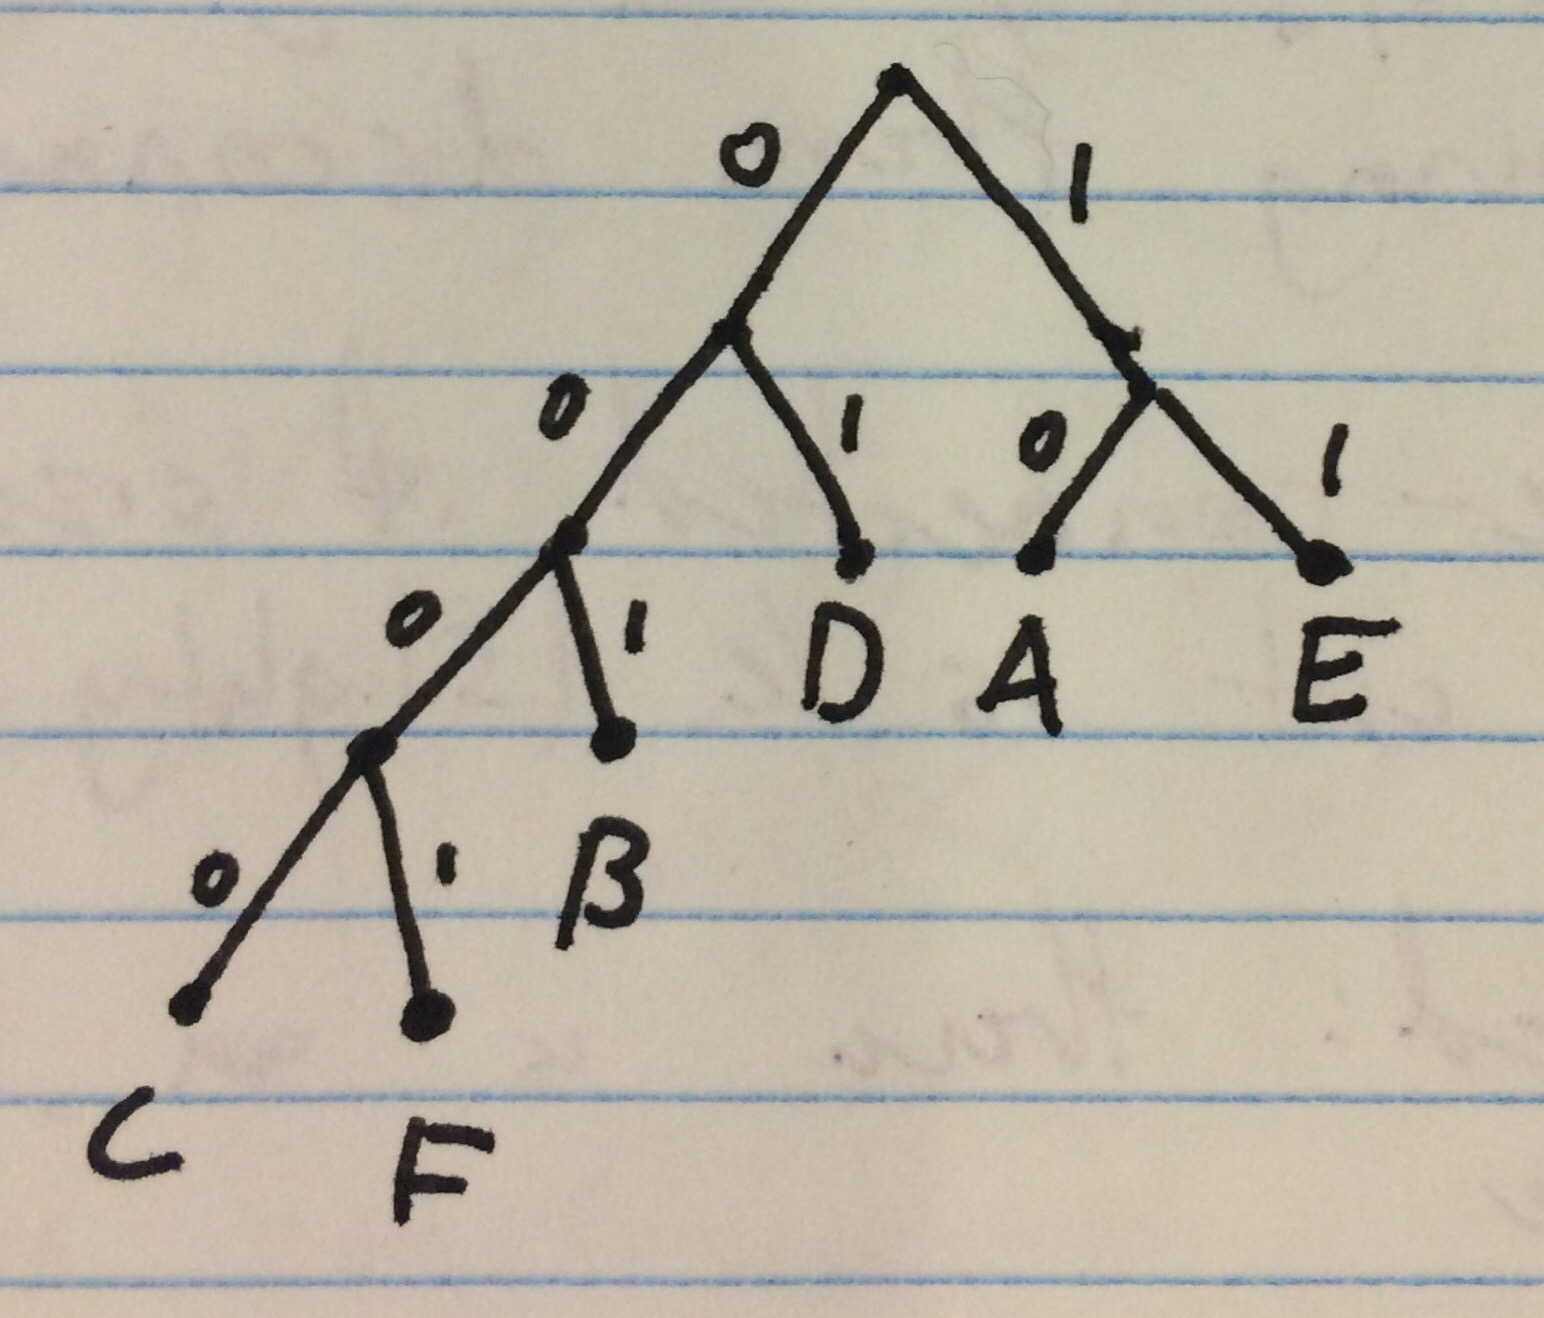
\includegraphics[scale=0.25]{lec4-1}\\
\\
\underline{Input:} $\Gamma (n = |\Gamma|)$ and $\forall x, f(x) = $frequency of $x$ such that $$\sum_{x\in\Gamma} f(x) =1$$

\underline{Output:} A Binary Tree $T$ that minimizes: $$AD(T) = \sum_{x\in\Gamma} f(x)\cdot \text{depth}_T(x) \:\:\:\text{(Average depth)}$$

\underline{Example:}\\
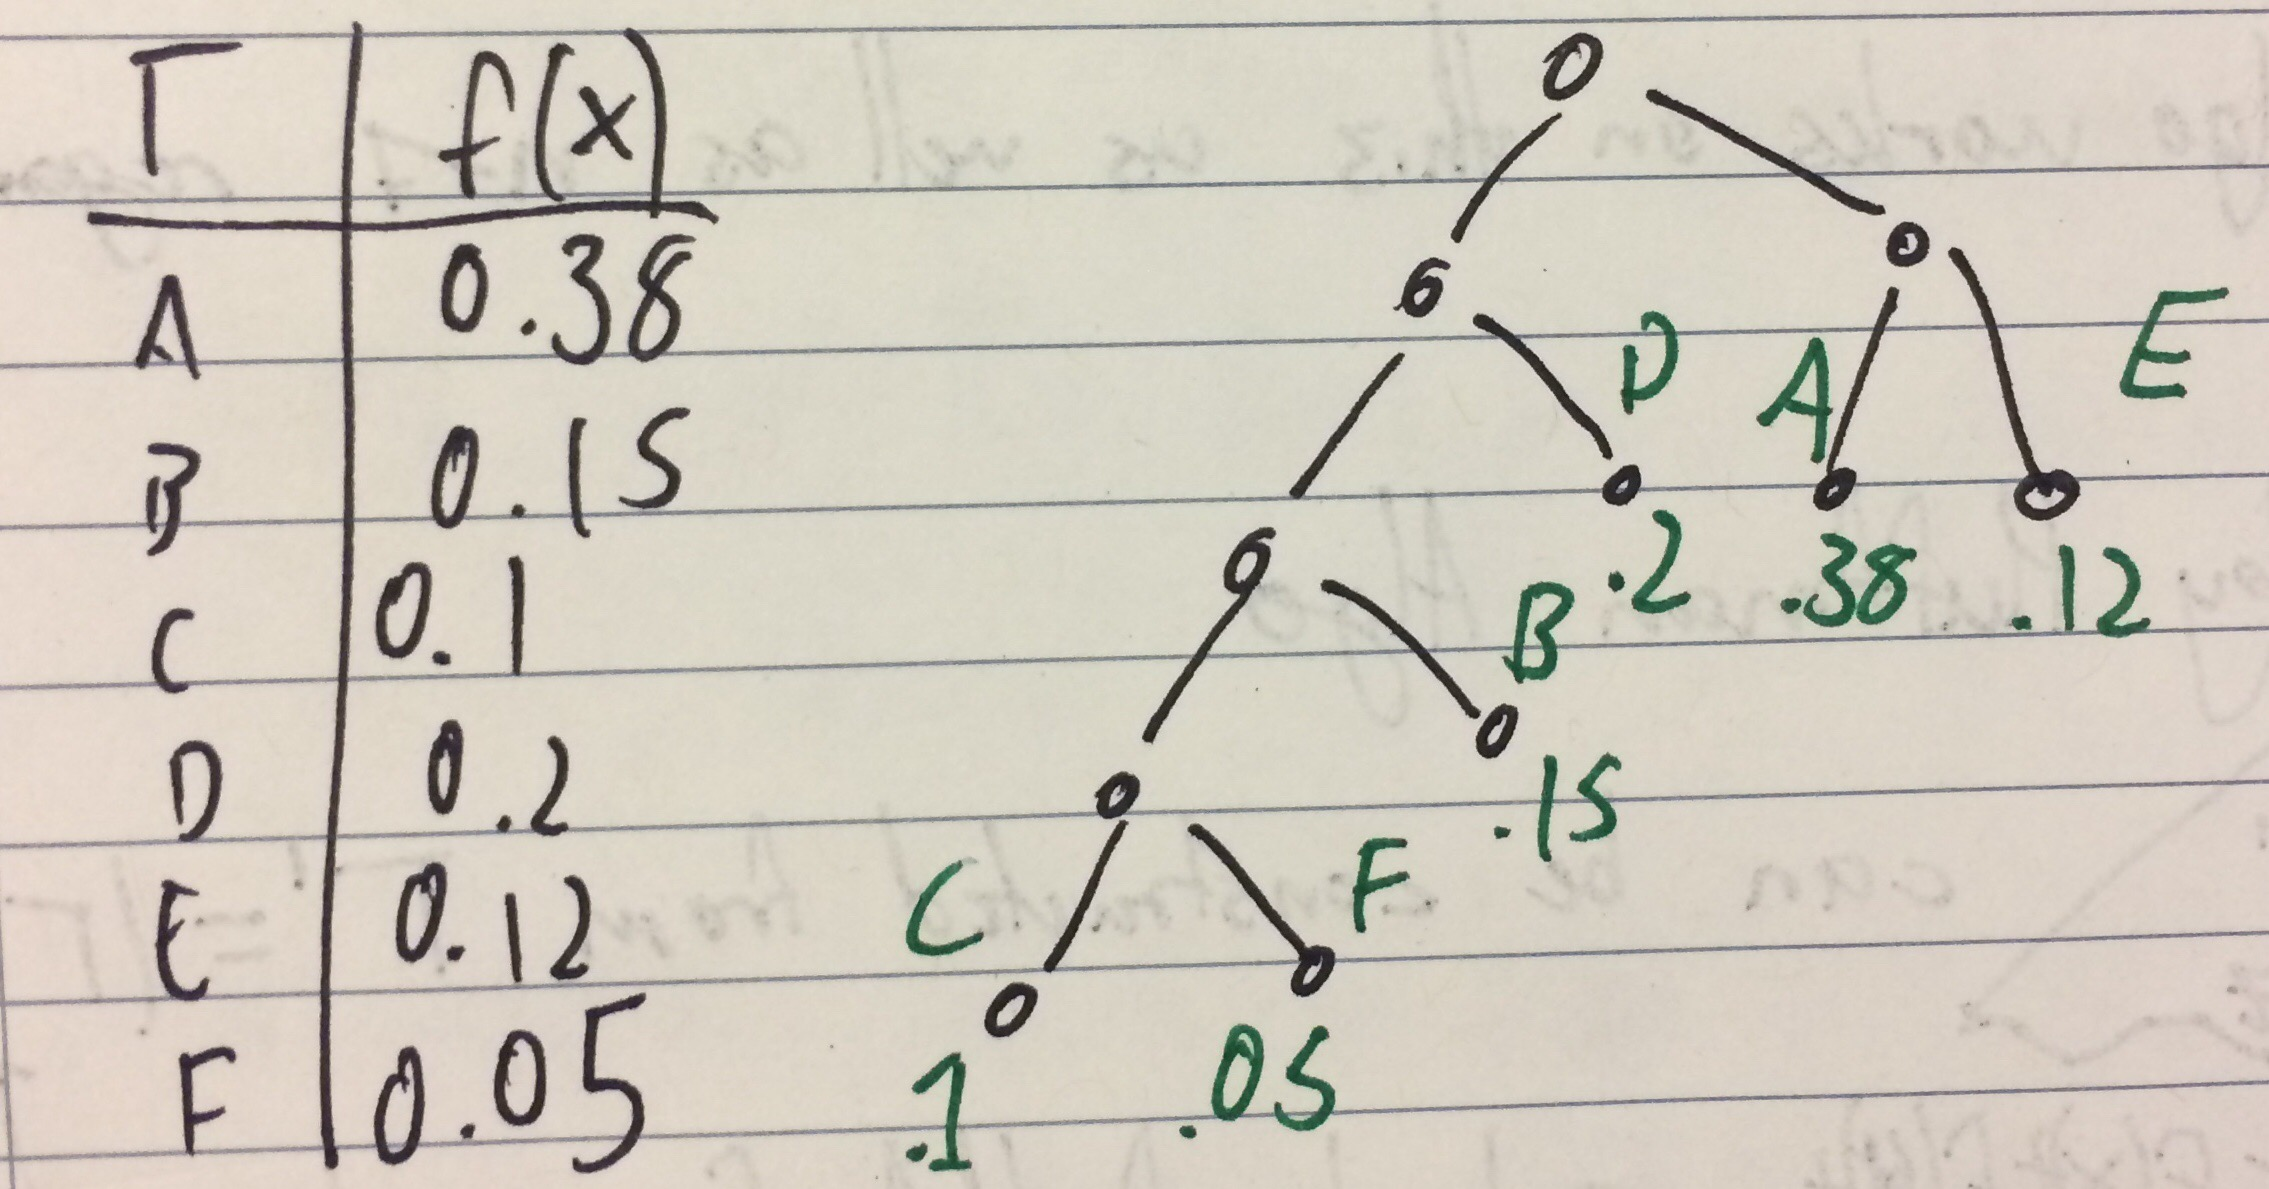
\includegraphics[scale=0.125]{lec4-2}

$$AD(T) = 4(.1 + .05) + 3(.15) + 2(.2 + .38 + .12) = 2.45$$

In this example, we would need 3 for a fixed length code (in bits), so this variable length code is good, but not optimal, must give more frequent letters for smaller codes.

\begin{tcolorbox}
	\underline{Note:}
	\begin{enumerate}
		\item{optimal trees must be full}
		\item{In an optimal $T$, $f(x) > f(y)$ implies that $\text{depth}_T (x) \leq \text{depth}_T (y)$}
	\end{enumerate}
\end{tcolorbox}

And both 1 and 2 notes imply that if $x,y\in\Gamma$ are minimum frequency then there exists an optimal tree such that $x,y$ are both siblings at max depth of $T$.

\subsubsection{Algorithm Intuition}

\begin{itemize}
	\item{Create leaves for all symbols}
	\item{Find 2 minimum frequency symbols $x,y$}
	\item{Make these children of a new node $z$}
	\item{remove x,y from $T$ and replace them by new "combined symbol" $z$, with the frequency equal to $f(x) + f(y)$}
	\item{Recursively build optimal tree for new set of symbols and frequency}
\end{itemize}

\subsubsection{Algorithm Correctness}

Now consider $|\Gamma| = n+1$ that the algorithm works on this as well as $n+1$ regardless of frequencies.\\
\\
Now let $H$ be a tree produced by the Huffman Algorithm.\\
\\
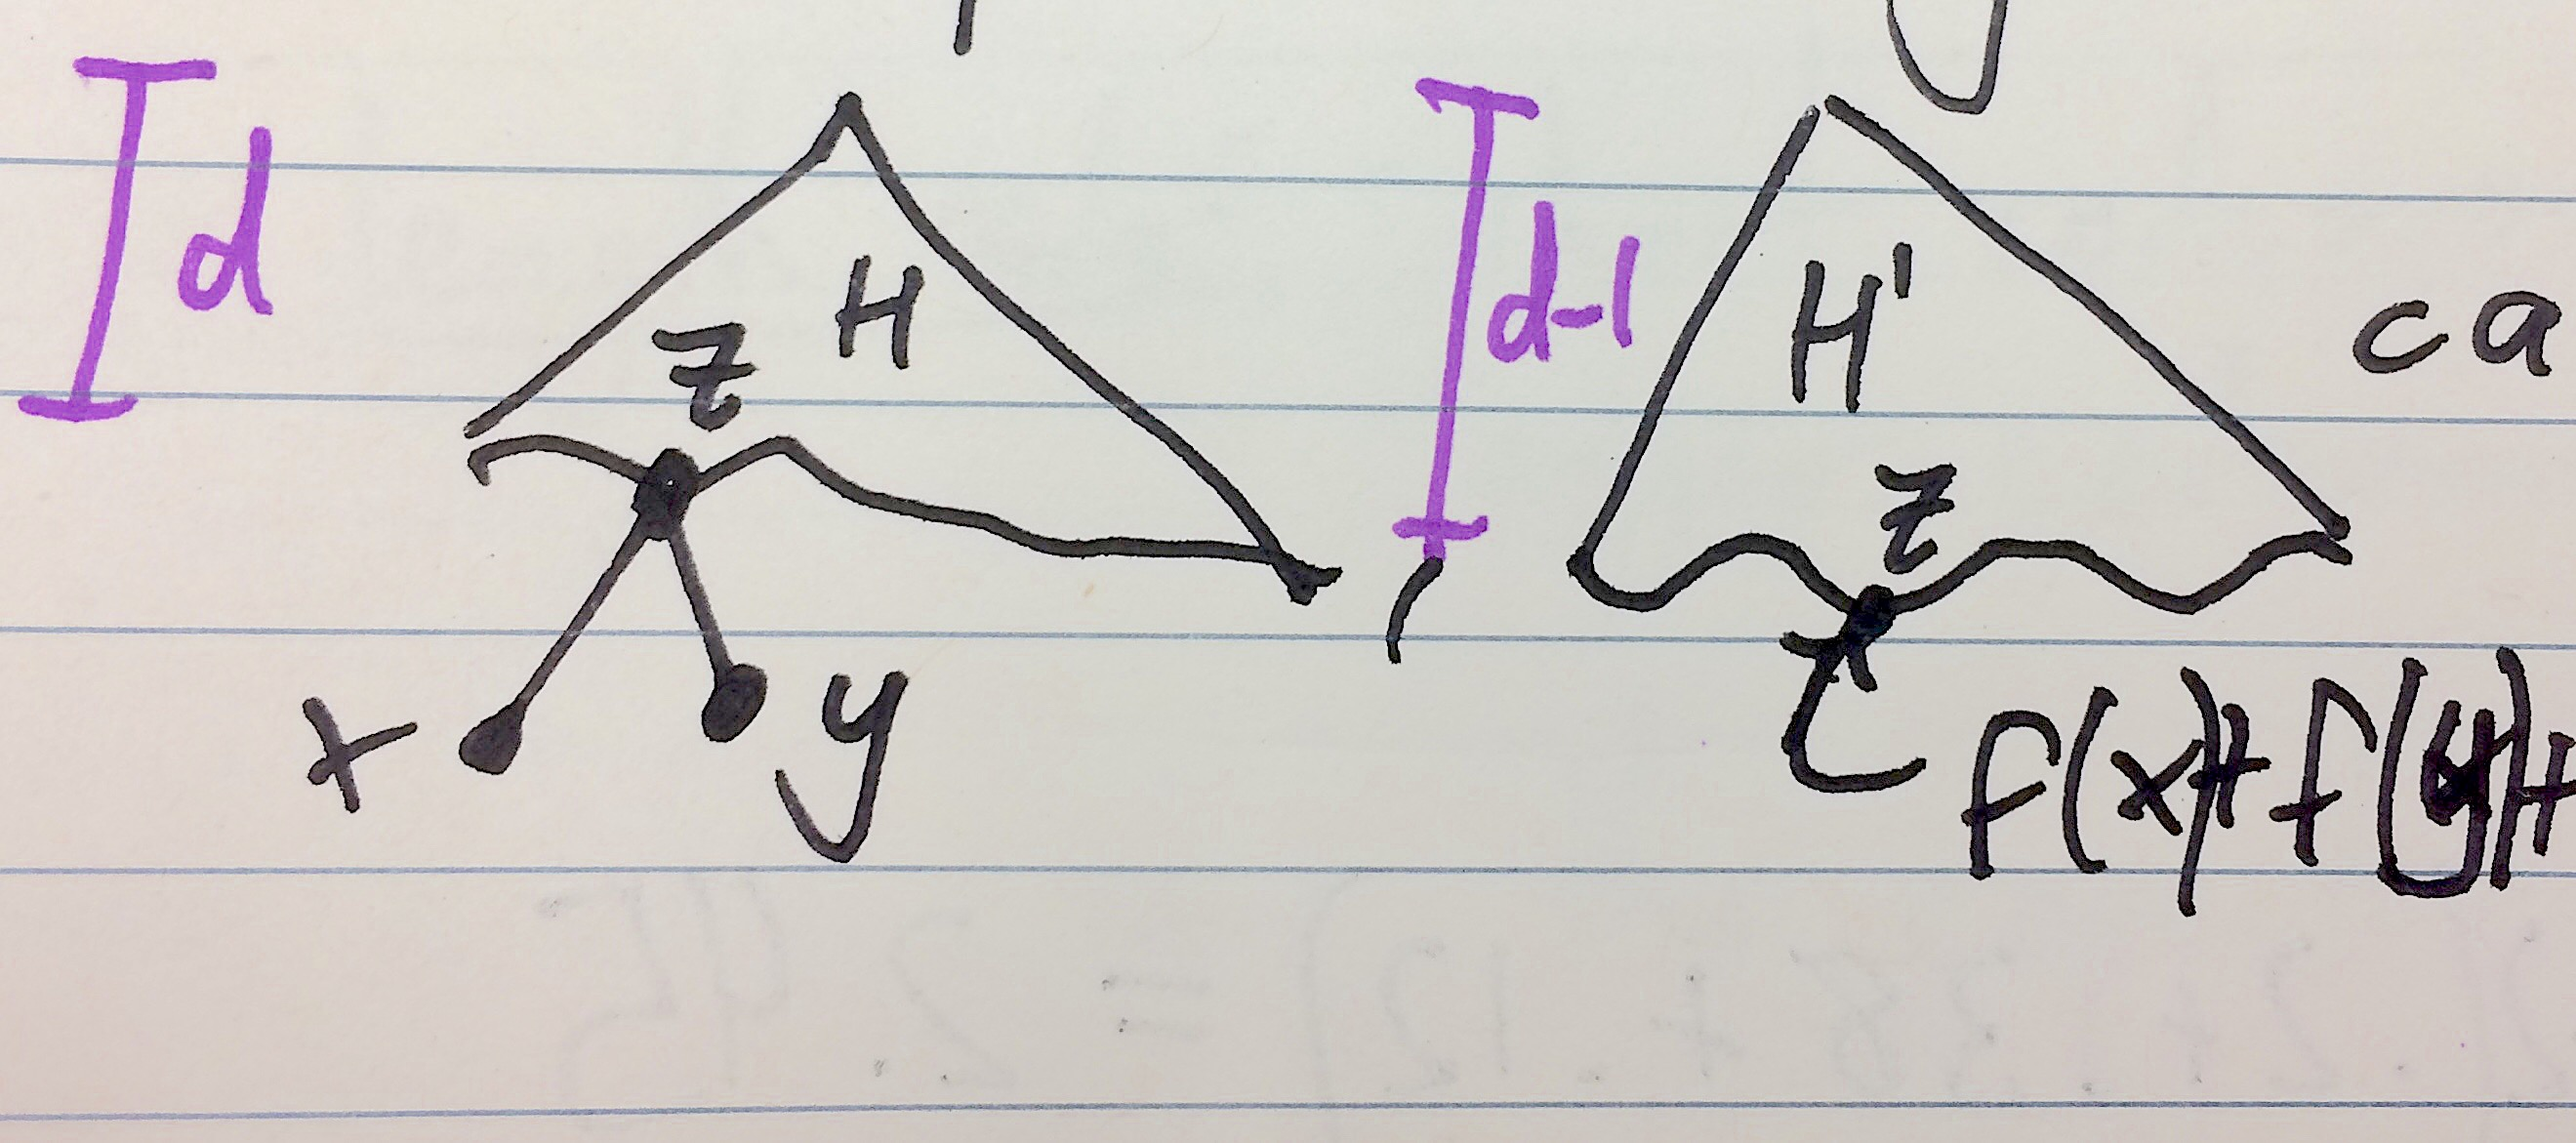
\includegraphics[scale=0.125]{lec4-3}
\\
\\
$H'$ can be constructed from $\Gamma' = (\Gamma - \{ x,y \}) \cup \{ z \}$. Note that $(\Gamma - \{ x,y \})$ is the Output of the Huffman Algorithm for input optimal by Induction Hypothesis.\\
\\
Now let $T$ be an optimal tree for $\Gamma, f$ by observations where $x,y$ are siblings at maximum depth. Consider $T'$ that is exactly like $T$ except $T'$ does not have $x,y$ nodes but their parent node $z$ with frequency $f(x) + f(y)$ remains as well.
\\
\\
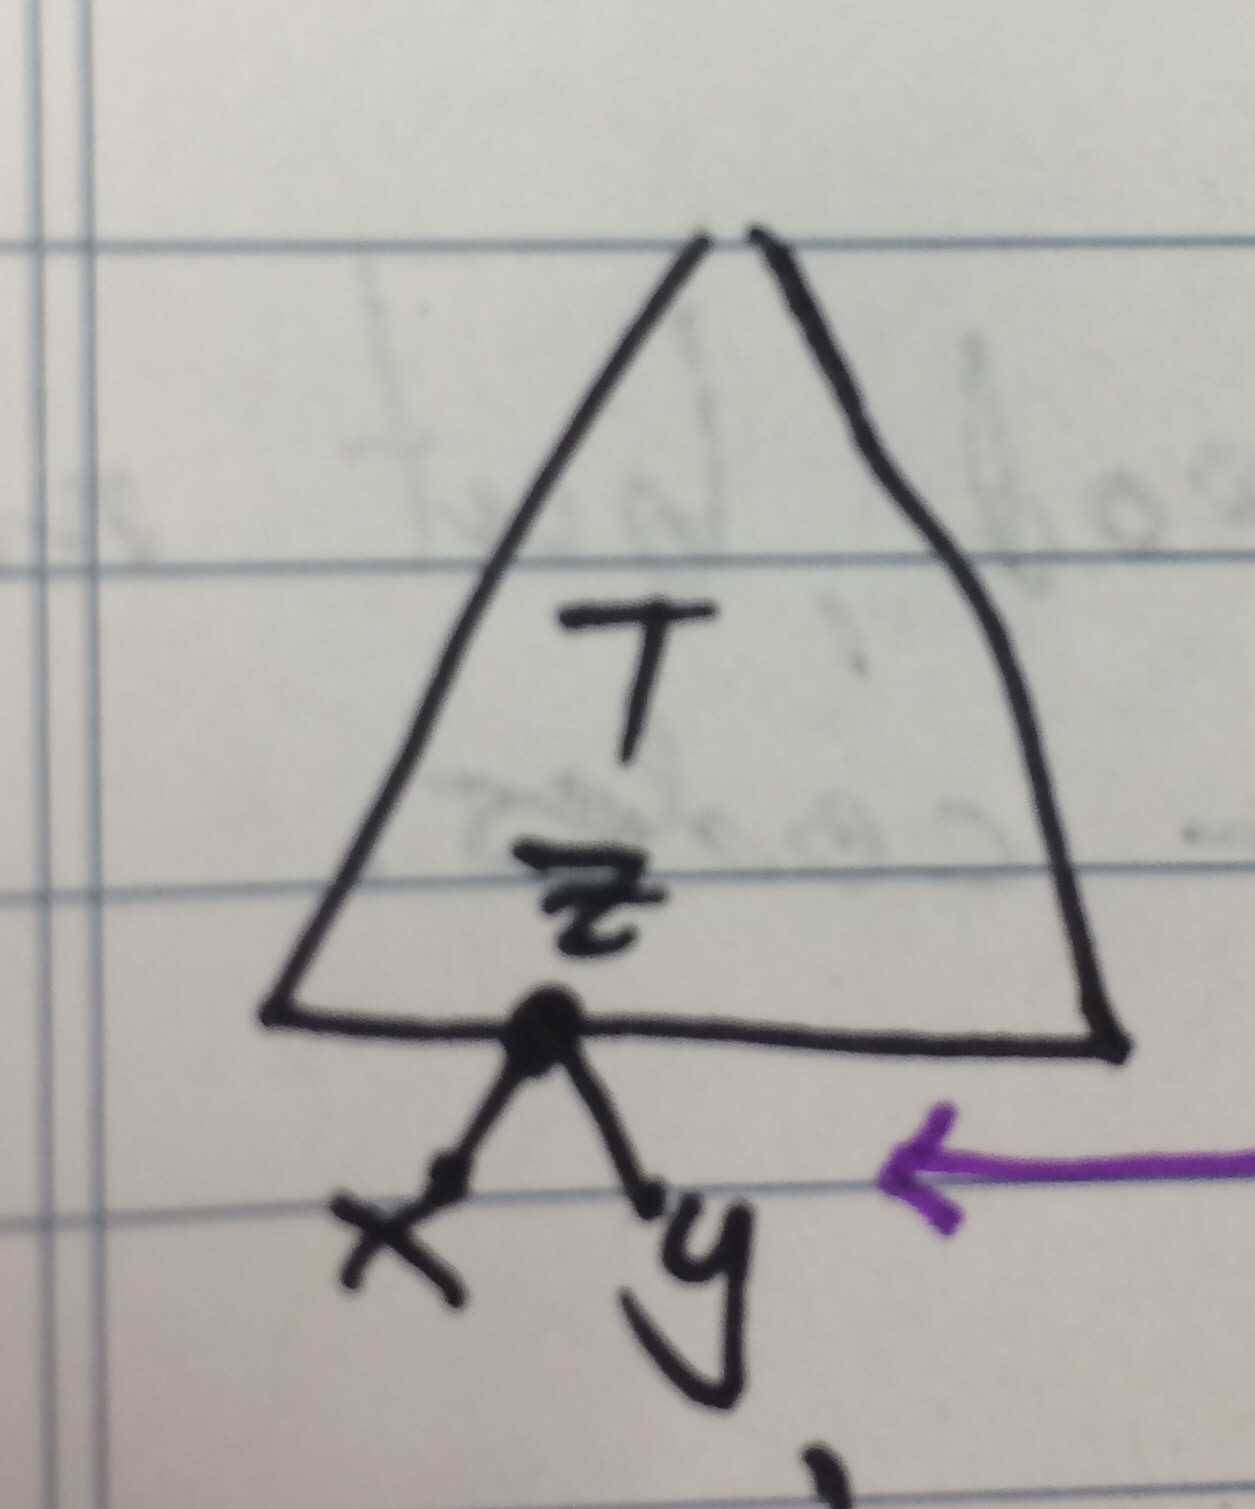
\includegraphics[scale=0.125]{lec4-4}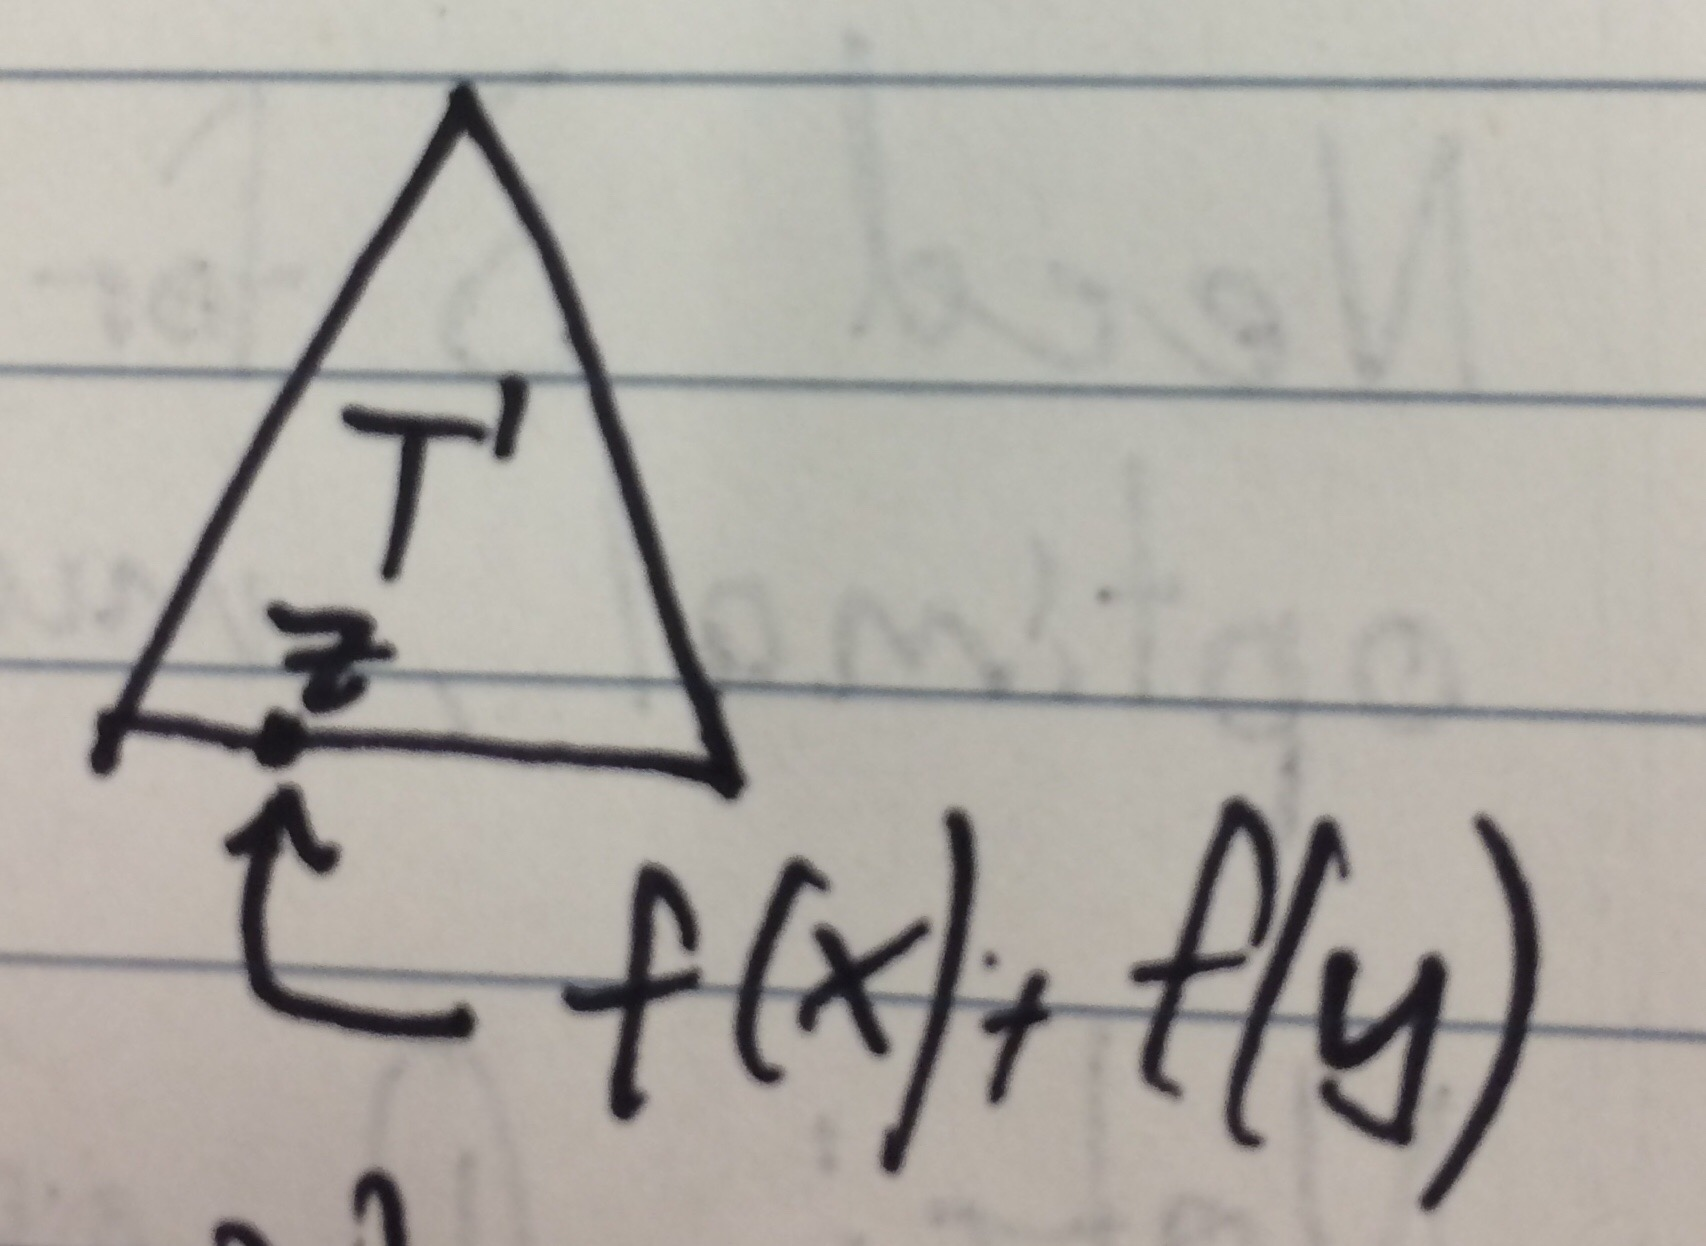
\includegraphics[scale=0.125]{lec4-5}
\\
\\
It follows that...
\begin{align*}
	AD(H) - AD(H') &= d(f(x) + f(y)) - (d-1)(f(x) + f(y))\\
	&= f(x)+f(y)\\
	AD(H) &= AD(H') + f(x) + f(y)\\
\end{align*}

and since...
$$AD(T) = AD(T) + f(x) + f(y)$$

\begin{align*}
	AD(H) &= AD(H') + f(x) + f(y)\\
	&= AD(T') + f(x) + f(y)\\
	&= AD(T)
\end{align*}

And since $T$ is optimal, it is implied that $H$ is optimal for $\Gamma, f$.\\
The Huffman Algorithm can also be implemented in $O(nlogn)$ time.

\newpage

\section{Wednesday, September 20, 2017}

\subsection{Divide and Conquer (DPV 2)(KT 5)}

\subsubsection{Mergesort}

To sort an array of $n$ elements\\
if $n=1$, trivial (already sorted)\\
else, divided array into two haves, recursively sort each half with Mergesort, then merge the two sorted halves.

\subsubsection{Binary Search}

To find $x$ in sorted array of $n$ elements\\
if $n=1$, trivial\\
else compare $x$ to middle element\\
	if $x\leq$ middle element, recursively search first half\\
	else, recursively search the second half
	
\subsubsection{General Divide and Conquer Template}

To solve an instance of size $n$ of some problem,\\
if $n$ is "small", solve directly\\
else
\begin{itemize}
	\item{split input into $a$ pieces, each of size $\frac{n}{b}$ for some $a\geq 1, b>1$ (constants that do not depend on $n$)}
	\item{recursively solve each of $a$ subproblems of size $\frac{n}{b}$}
	\item{combine solution to subproblems into for original instance of problems}
\end{itemize}

\begin{tcolorbox}
	if problem of size $n$ is broken down and a recursive call is called on a problem of size $\frac{n}{b}$, then this is considered as a divide and conquer algorithm.\\
	\\
	if problem of size $n$ is broken down and a recursive call is called on a problem of size $n-c$ where $c$ is a constant, then this is not considered as a divide and conquer algorithm.
\end{tcolorbox}

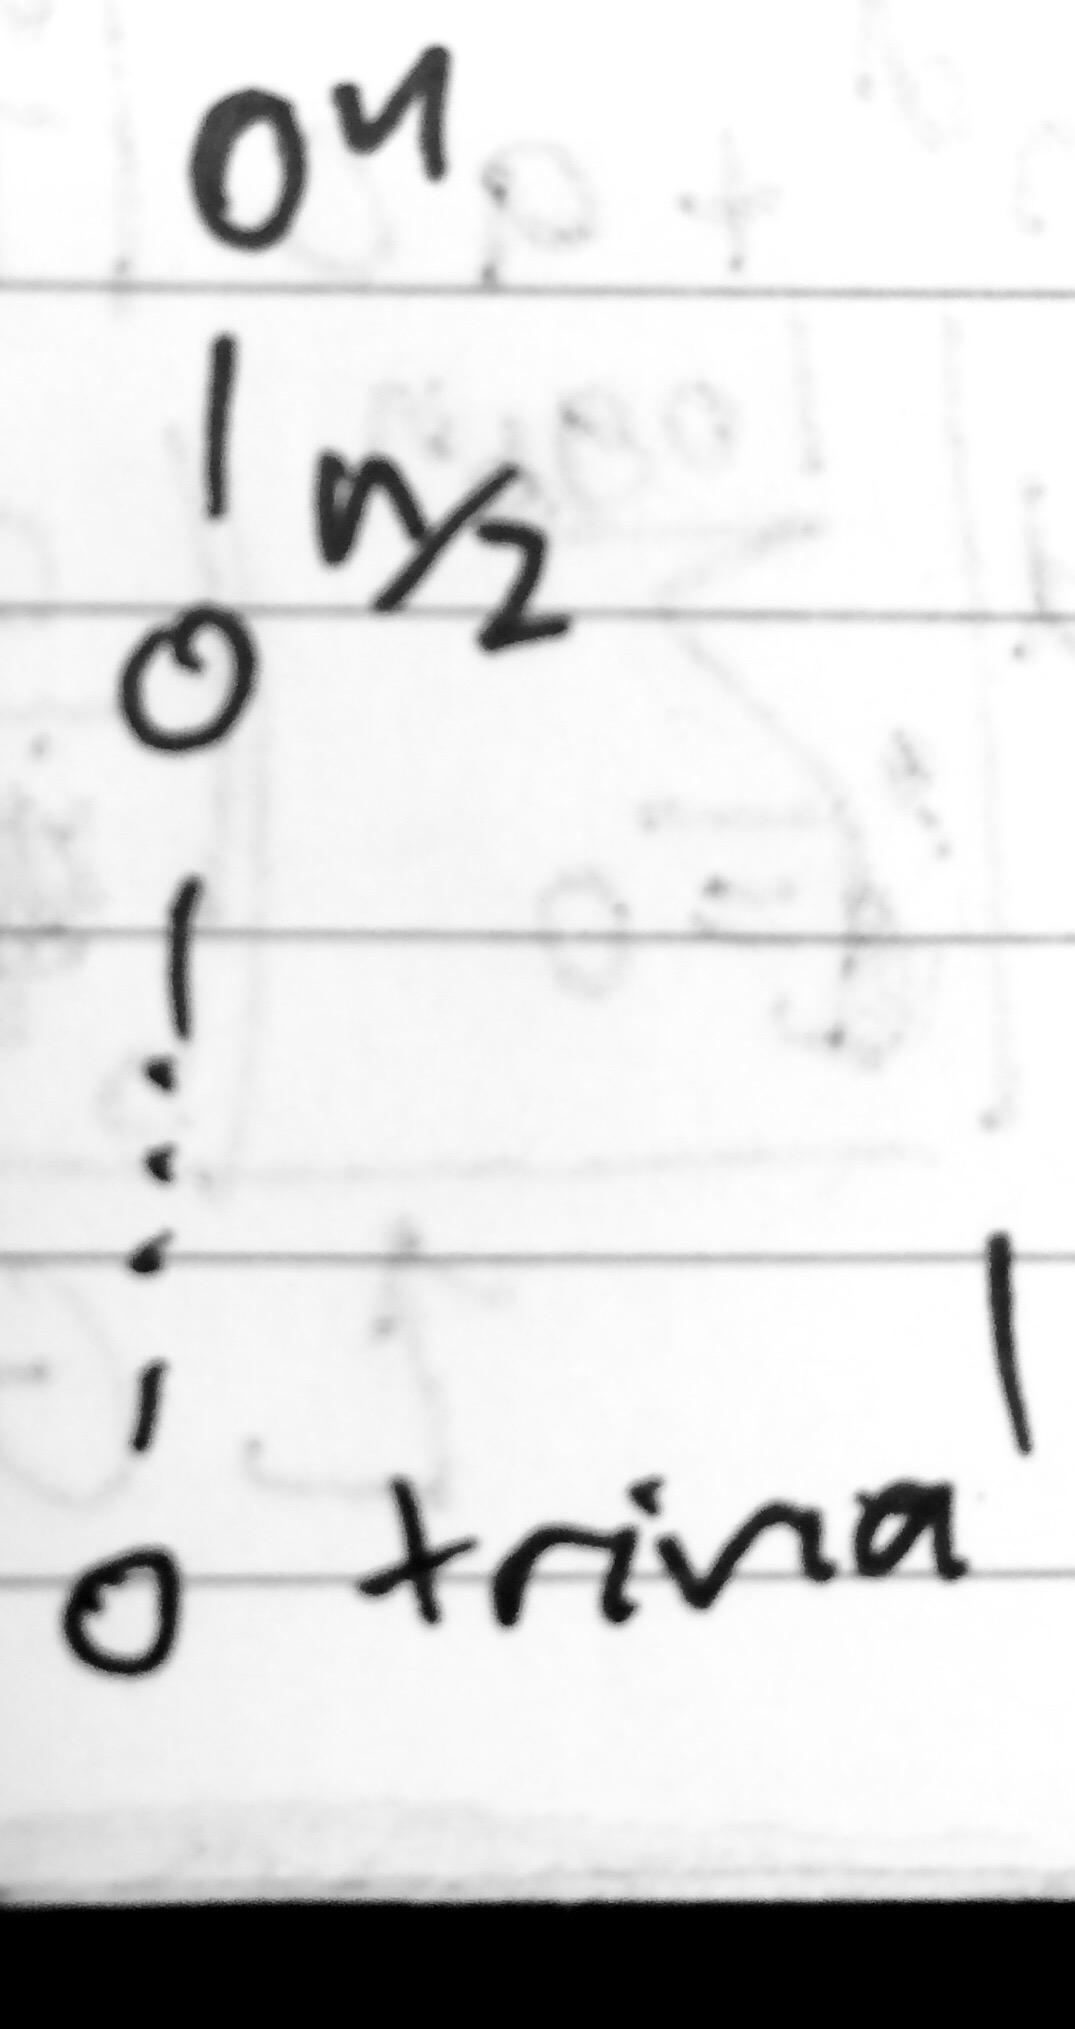
\includegraphics[scale=0.08]{lec5-1}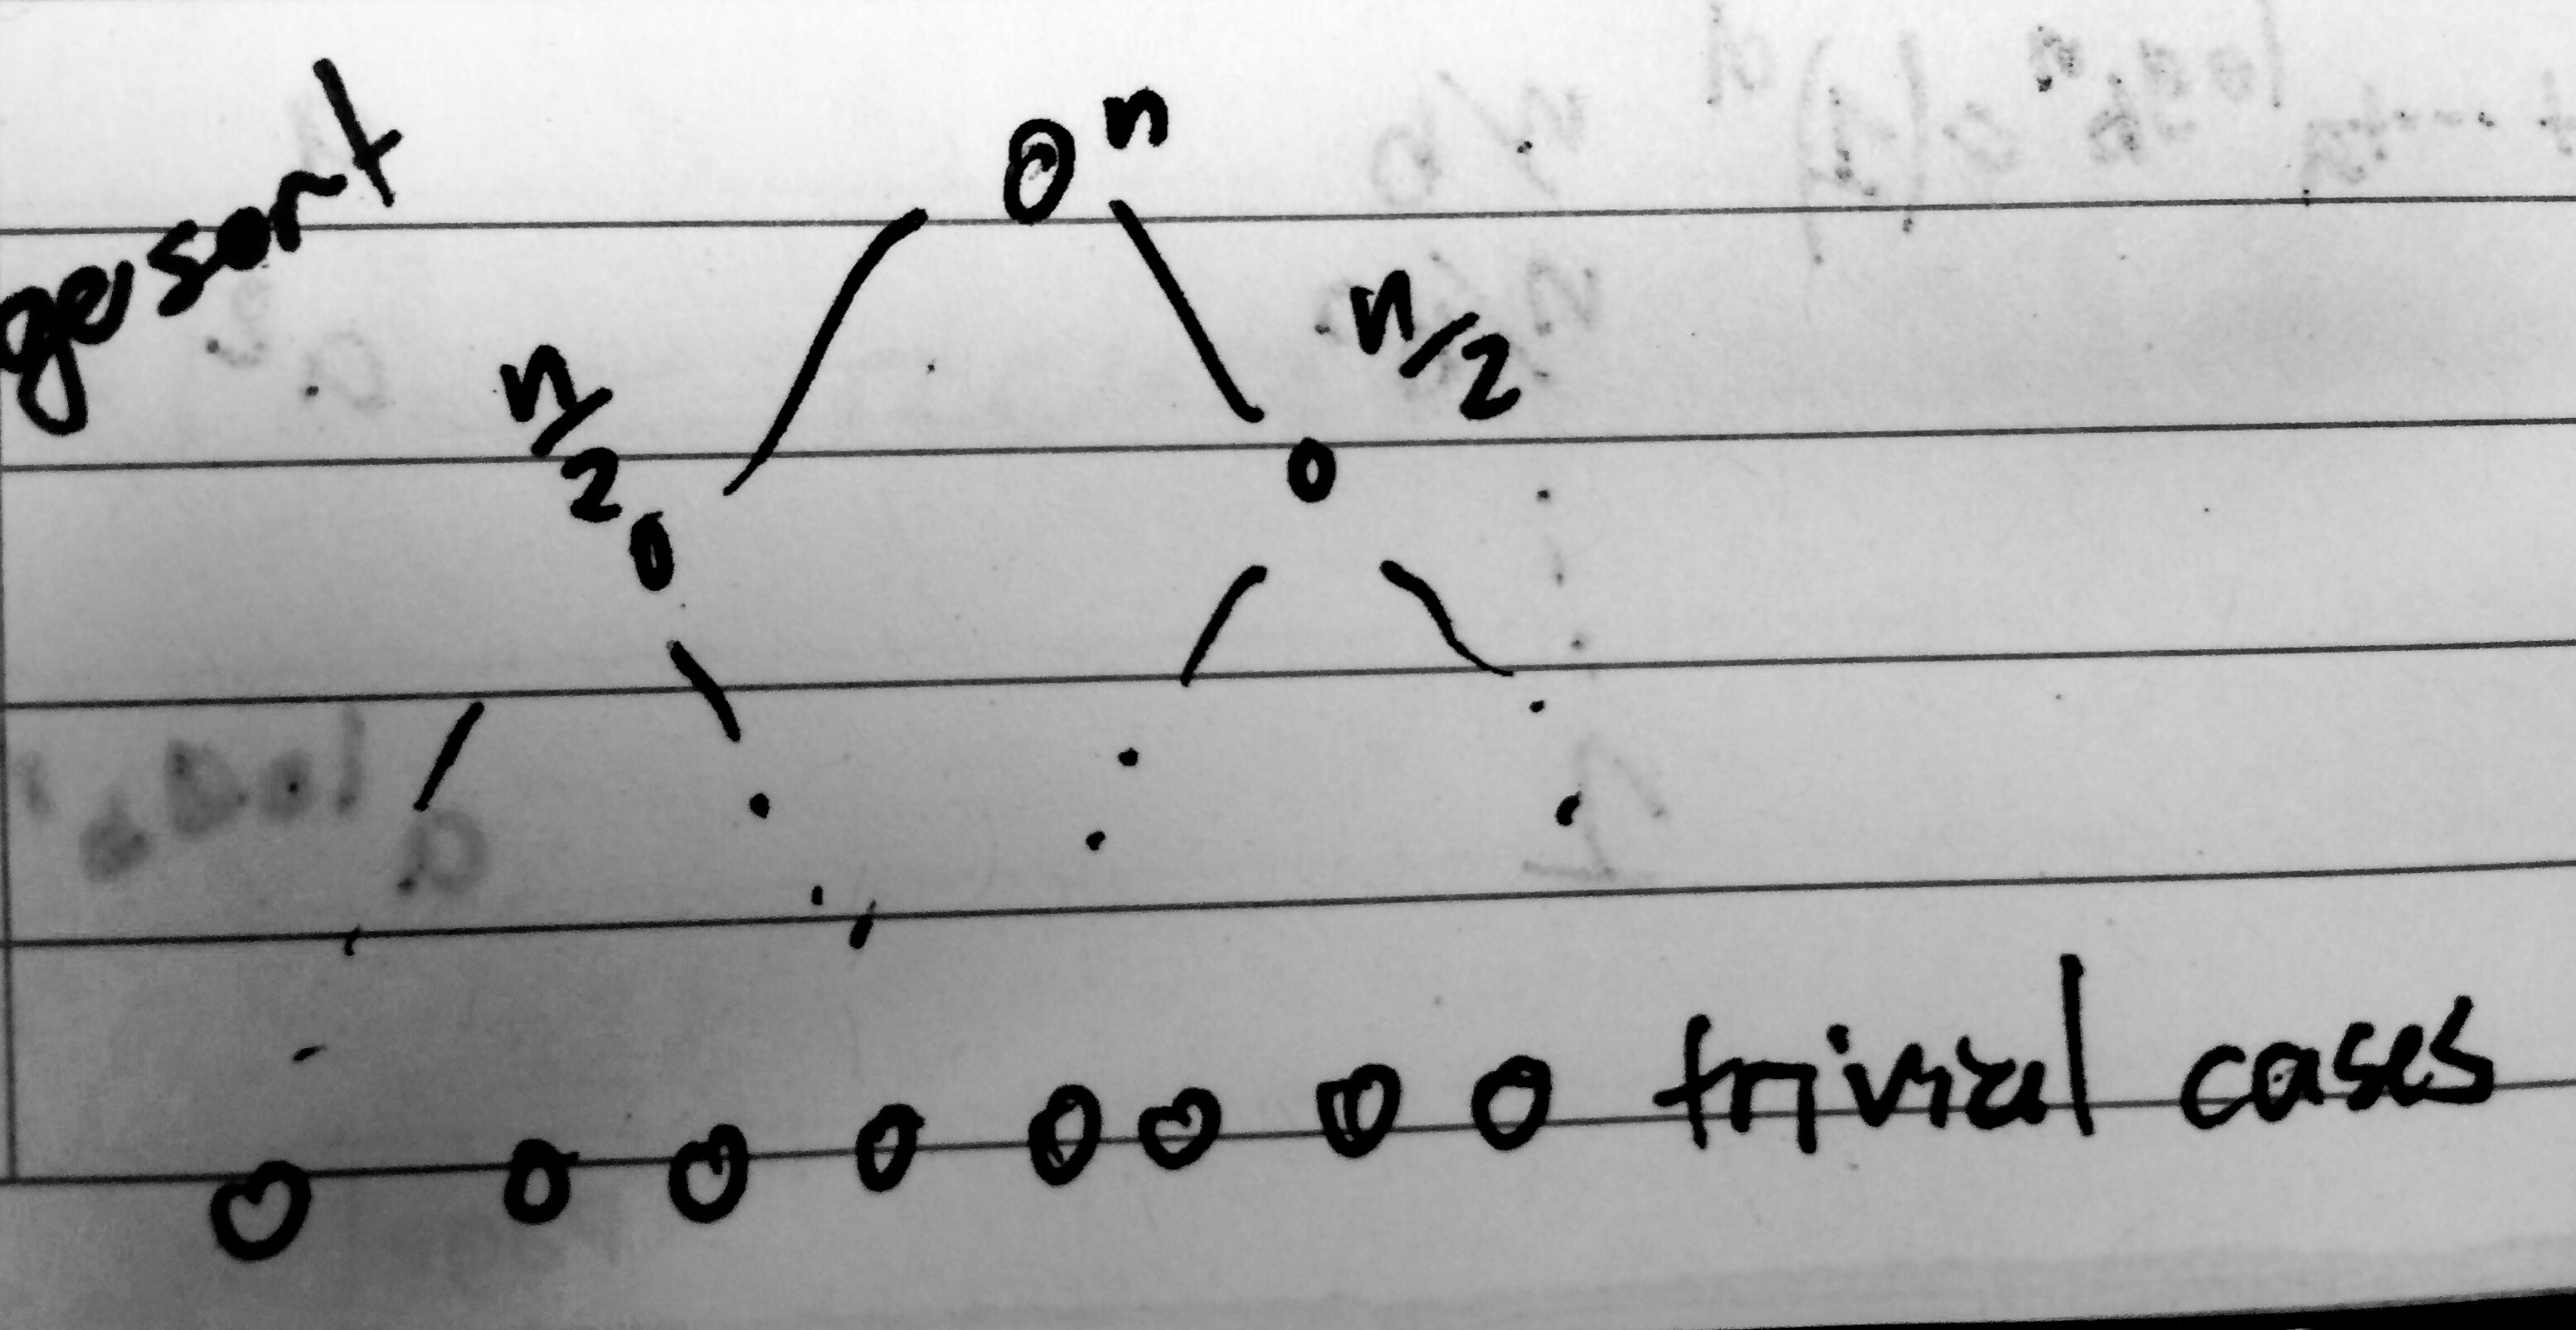
\includegraphics[scale=0.1]{lec5-2}
(Binary Search and Mergesort cases visualized)

\subsubsection{General Structure for Divide and Conquer Algorithms}

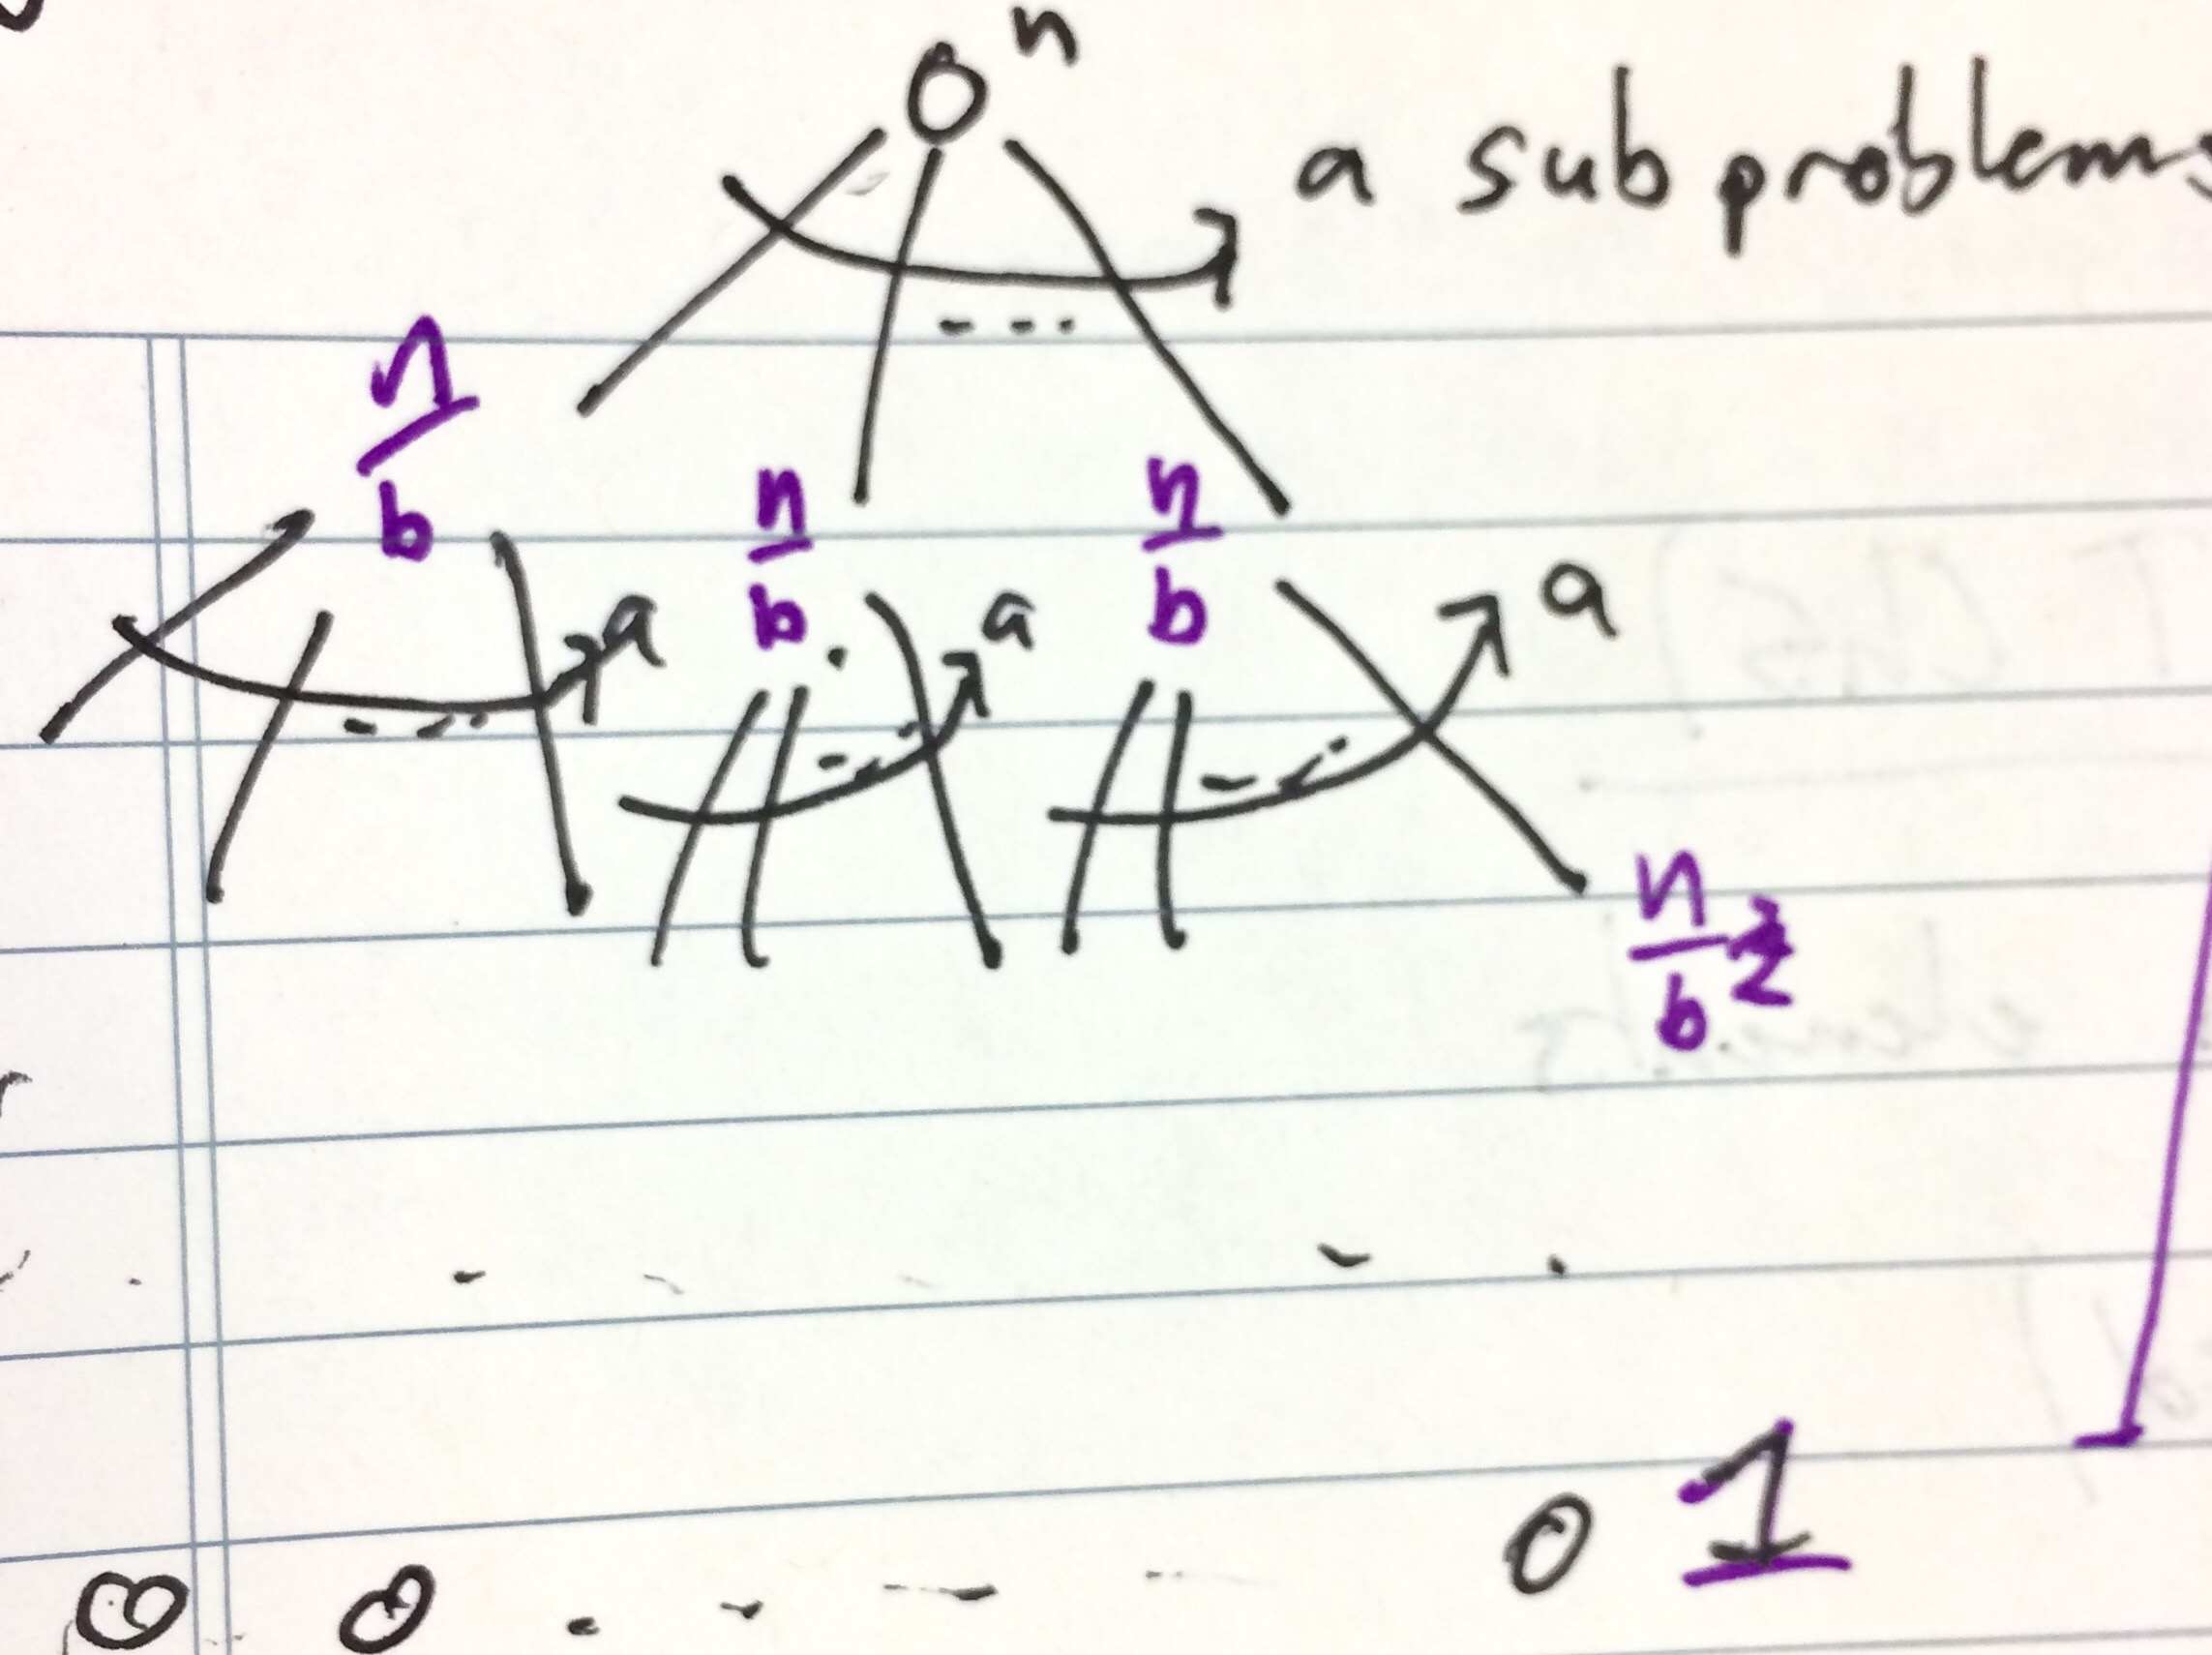
\includegraphics[scale=0.1]{lec5-3}\\
($log_b n$ levels of a divide and conquer algorithms visualized)

\subsubsection{Recurrence to Describe Running Time of Divide and Conquer Algorithms}

\underline{e.g.}
\begin{itemize}
	\item{Merge Sort $T(n) = 2T(\frac{n}{2})+cn$ implies that $T(n) = \Theta (nlogn)$ by repeated substitution}
	\item{Binary Search $T(n) = T(\frac{n}{2})+c$ implies that $T(n) = \Theta (logn)$ by repeated substitution}
\end{itemize}

\subsubsection{Recurrence for "Generic" Divide and Conquer Algorithms}

$$T(n) = aT(\frac{n}{b}) + cn^d$$
$aT(\frac{n}{b})$ refers to the time spent on recursive calls and $cn^d$ refers to time splitting input and combining results of small instances

\subsubsection{"Master Theorem" for $T(n)$ as defined previously}

\begin{enumerate}[label=\alph*]
	\item{if $a < b^d$ then $T(n) = \Theta (n^d)$}
	\item{if $a = b^d$ then $T(n) = \Theta (n^d)$}
	\item{if $a > b^d$ then $T(n) = \Theta (n^d)$}
\end{enumerate}

\begin{proof}(Proof for the entire Master Theorem)\\
\\
Assume $n$ is a power of $b$.

\begin{align*}
	T(n) &= (1)cn^d + ac(\frac{n}{b})^d + a^2 c (\frac{n}{b^2})^d + ... + a^{log_b n} c (1)^d\\
	&= cn^d + \sum^{log_b n}_{i=0} (\frac{a}{b^d})^i\\
	&= cn^d + G(n)
\end{align*}

\underline{Recall that:} $$1+x+x^2 + ... + x^k = \frac{x^{k+1}-1}{x-1}$$
$$1+x+x^2 + ... = \frac{1}{x-1}, \forall x<1$$

\underline{a} $$a<b^d \longrightarrow \frac{a}{b^d} < 1$$
$$G(n) \leq \sum^\infty_{i=0} (\frac{a}{b^d})^i = \frac{1}{1-\frac{a}{b^d}} = \Theta (1)$$
This implies that $T(n) = cn^d\Theta (1) = \Theta (n^d)$
\\
\\
\underline{b}
$$a = b^d \text{ implies that } \frac{a}{b^d} = 1 \text{ which implies that } G(n) = 1+ log_b n = \Theta (log_b n)$$
$\text{ which finally implies that } T(n) = cn^d\Theta (logn) = \Theta (n^d logn)$\\
\\
\underline{c}
$$a > b^d \longrightarrow \frac{a}{b^d} > 1$$
\begin{align*}
	G(n) &= \sum^{log_b n}_{i=0} (\frac{a}{b^d})^i\\
	&= \frac{(a/b^d)^{1+log_b n}-1}{(a/b^d)-1}\\
	&= \frac{(a/b^d)(a/b^d)^{log_b n}-1}{(a/b^d)-1}\\
	&= \Theta ((a/b^d)^{log_b n})\\
	&= \Theta (\frac{a^{log_b n}}{(b^{log_b n})^d})\\
	&= \Theta (\frac{n^{log_b a}}{n^d})
\end{align*}

This implies that $T(n) = cn^d \Theta (\frac{n^{log_b a}}{n^d}) = \Theta (n^{log_b a})$

\end{proof}

\begin{tcolorbox}[title=Intuition]
	\begin{enumerate}[label=\alph*]
	\item{$cn^d$ dominates the function}
	\item{both factors weigh into running time}
	\item{other recursive calls dominate the function}
\end{enumerate}
\end{tcolorbox}

\subsection{Karatsuba's Multiplication Algorithm}

Can do addition in $\Theta (n)$ time or $\Theta (n)$ bit operations.

\subsubsection{Classic Algorithm for Multiplication}

Multiplying and then bit shifting, $n^2$ multiplications $+ (n-1)$ additions of $\leq 2n$ bit numbers resulting in $\Theta (n^2)$

\subsubsection{Divide and Conquer Idea \# 1}

take 2 $n$-bit numbers $X,Y$ and divide them into two sections such that
$$X = X_1 2^{(n/2)} + X_0$$
$$Y = Y_1 2^{(n/2)} + Y_0$$

so we know that
$$XY = X_1 Y_1 2^n + (X_1 Y_0 + X_0 Y_1) 2^{(n/2)} + X_0 Y_0 $$

$T(n) = 4T(\frac{n}{2}) +cn, a=4, b=2, d=1$, and since $4 > 2^1$, case (c) applies.\\
So $T(n) = \Theta (n^{log_2 n}) = \Theta (n^2)$ which literally does nothing to improve complexity.

\subsubsection{Divide and Conquer Idea \# 2}

$$XY = X_1 Y_1 2^n + ((X_1 + X_0)(Y_1 + Y_0) - X_1 Y_1 - X_0 Y_0) 2^{n/2} + X_0 Y_0$$

$T(n) = 3 T(\frac{n}{2}) + cn, a=3, b=2, d=1$ and since $3 > 2^1$, this implies that case (c) applies and so $T(n) = \Theta (n^{log_2 3}) = \Theta (n^{1.565})$\\
\\
Consider addition of $X_0$ and $X_1$, the result will be a new number of $v_0$ which is $n/2$ bits, with another carry at the end of this number $v_1$ which is a one bit number. The same thing is the result for $Y_0$ and $Y_1$, which also results in a $\frac{n}{2} + 1$ bit number.\\
\\
Because of this we know that multiplication can be considered by $2(\frac{n}{2})$ bits and a linear amount of work.

\subsubsection{Algorithm for Divide and Conquer Idea \# 2}

\begin{lstlisting}[language=Python]
MULT(x,y): #x,y must both be boolean arraw of length of at least 1
	n := max(length(x), length(y))
	if n=1 then do
		return (x[1] or y[1])
	else
		put n-length(x) 0s to the left of x
		put n-length(y) 0s to the left of y
		
		x1 := leftmost n/2 bits of X
		x0 := rightmost n/2 bits of X
		y1 := leftmost n/2 bits of Y
		y0 := rightmost n/2 bits of Y
		
		s := ADD(x1, x0) # s = x0 + x1
		t := ADD(y1, y0) # t = y0 + y1
		
		a := MULT(x1,y1) # a = (x1)(y1)
		b := MULT(x0,y0) # b = (x0)(y0)
		c := MULT(s,t) # c = (x1 + x0)(y1 + y0)
		
		u : SUB(c,ADD(a,b)) # u = c - a - b
		
		put n 0s to the right of a
		put n/2 0s to the right of u
		
		return ADD(a, ADD(u,b))
\end{lstlisting}

\subsubsection{Applying the Master Theorem}

I honestly have no idea why this is here, but I guess this is just an example of how you can use the master theorem to find the complexity of some popular algorithms:

\paragraph{Merge Sort} $a=2, b=2, d=1$ and since $2 = 2^1$ then Merge Sort has a time complexity of $\Theta (nlogn)$

\paragraph{Binary Search} $a=1, b=2,d=0$ and since $1 = 2^0$ then Binary Search has a time complexity of $\Theta (logn)$

\subsection{Celebrity Problem}

Everyone in a bar knows a celebrity in the bar, but the celebrity knows no one. You enter the bar and must find the celebrity by only asking: "Do you (Person $A$) know Person $B$?".\\
\\
Can you find the celebrity with the least number of questions given $n$ people in the bar?

\begin{tcolorbox}
	\underline{Note:} After every question, if the person says yes, you know that Person $A$ is not the celebrity, but if the person says no, you know that Person $B$ is not the celebrity.
\end{tcolorbox}

\newpage


\end{document}


























